\documentclass{whiteboard}
\begin{document}
\begin{frame}[plain,t]
\bbcover{Grafos}{Ordenação Topológica}{Prof. Edson Alves}{Faculdade UnB Gama}

\end{frame}
\begin{frame}[plain,t]
\begin{tikzpicture}
\node[draw,opacity=0] at (0, 0) {x};
\node[draw,opacity=0] at (14, 8) {x};

	\node[anchor=west] (title) at (0.0, 6.0) { \Large \bbbold{Ordenação topológica} };
\end{tikzpicture}
\end{frame}
\begin{frame}[plain,t]
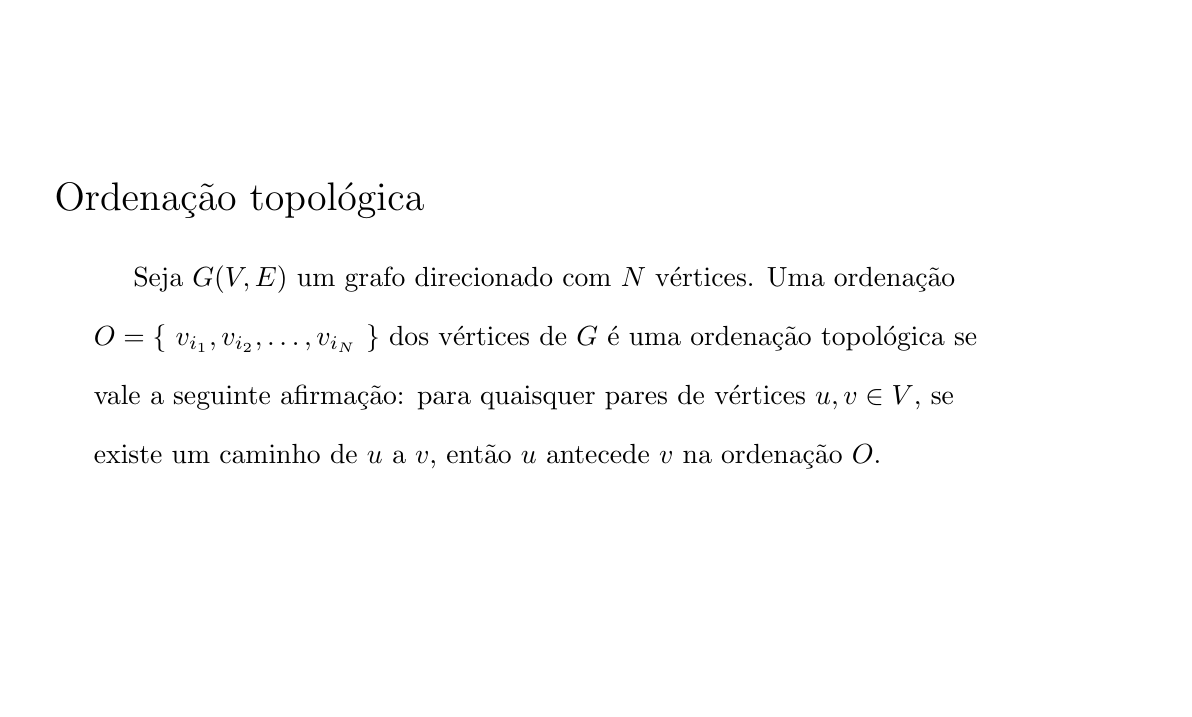
\begin{tikzpicture}
\node[draw,opacity=0] at (0, 0) {x};
\node[draw,opacity=0] at (14, 8) {x};

	\node[anchor=west] (title) at (0.0, 6.0) { \Large \bbbold{Ordenação topológica} };

	\node[anchor=west] (a) at (1.0, 5.0) { \bbtext{Seja $G(V, E)$ um grafo direcionado com $N$ vértices. Uma ordenação } };

	\node[anchor=west] (b) at (0.5, 4.25) { \bbtext{$O = \{\ v_{i_1}, v_{i_2}, \ldots, v_{i_N}\ \}$ dos vértices de $G$ é uma \bbbold{ordenação topológica} se} };

	\node[anchor=west] (c) at (0.5, 3.5) { \bbtext{vale a seguinte afirmação: para quaisquer pares de vértices $u, v \in V$, se } };

	\node[anchor=west] (d) at (0.5, 2.75) { \bbtext{existe um caminho de $u$ a $v$, então $u$ antecede $v$ na ordenação $O$.} };

\end{tikzpicture}
\end{frame}
\begin{frame}[plain,t]
\begin{tikzpicture}
\node[draw,opacity=0] at (0, 0) {x};
\node[draw,opacity=0] at (14, 8) {x};

	\node[anchor=west] (title) at (0.0, 7.0) { \Large \bbbold{Características da ordenação topológica} };
\end{tikzpicture}
\end{frame}
\begin{frame}[plain,t]
\begin{tikzpicture}
\node[draw,opacity=0] at (0, 0) {x};
\node[draw,opacity=0] at (14, 8) {x};

	\node[anchor=west] (title) at (0.0, 7.0) { \Large \bbbold{Características da ordenação topológica} };

	\node[anchor=west] (a) at (1.0, 6.0) { $\star$ \bbtext{Grafos que possuem ciclos não possuem ordenações topológicas} };

\end{tikzpicture}
\end{frame}
\begin{frame}[plain,t]
\begin{tikzpicture}
\node[draw,opacity=0] at (0, 0) {x};
\node[draw,opacity=0] at (14, 8) {x};

	\node[anchor=west] (title) at (0.0, 7.0) { \Large \bbbold{Características da ordenação topológica} };

	\node[anchor=west] (a) at (1.0, 6.0) { $\star$ \bbtext{Grafos que possuem ciclos não possuem ordenações topológicas} };


	\node[anchor=west] (b) at (1.0, 5.0) { $\star$ \bbtext{Um grafo direcionado acíclico (DAG) contém, no mínimo, uma ordenação } };

	\node[anchor=west] (b1) at (0.5, 4.5) { \bbtext{topológica} };

\end{tikzpicture}
\end{frame}
\begin{frame}[plain,t]
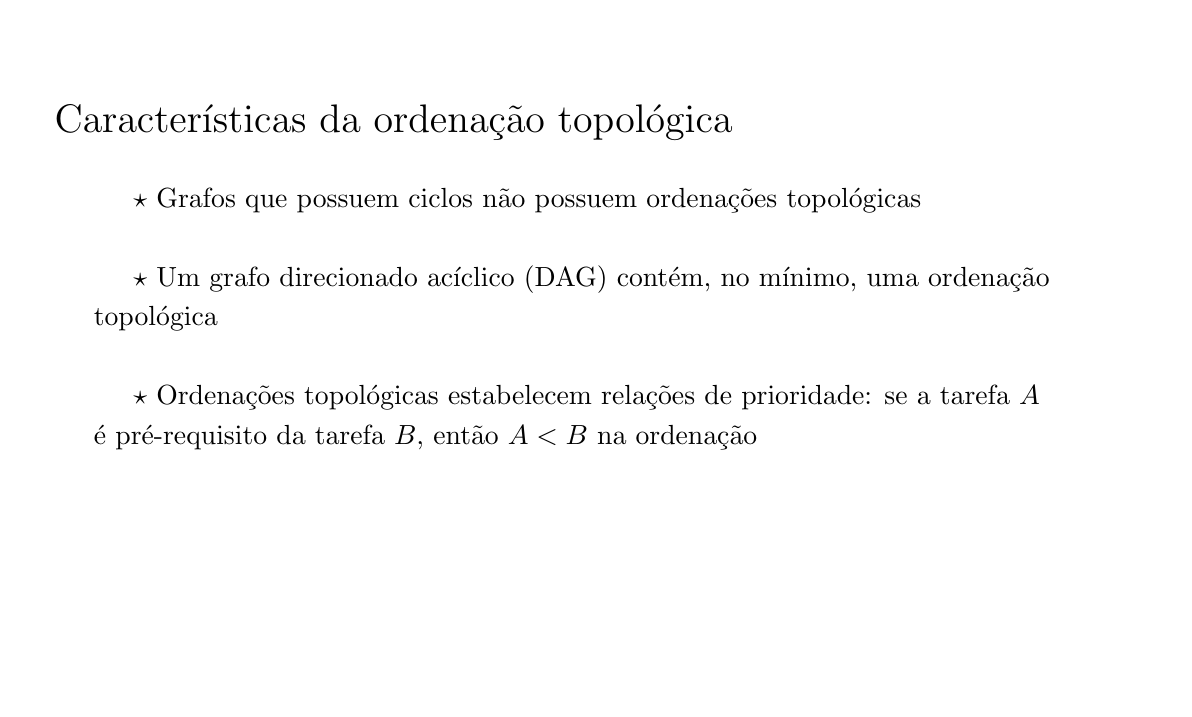
\begin{tikzpicture}
\node[draw,opacity=0] at (0, 0) {x};
\node[draw,opacity=0] at (14, 8) {x};

	\node[anchor=west] (title) at (0.0, 7.0) { \Large \bbbold{Características da ordenação topológica} };

	\node[anchor=west] (a) at (1.0, 6.0) { $\star$ \bbtext{Grafos que possuem ciclos não possuem ordenações topológicas} };


	\node[anchor=west] (b) at (1.0, 5.0) { $\star$ \bbtext{Um grafo direcionado acíclico (DAG) contém, no mínimo, uma ordenação } };

	\node[anchor=west] (b1) at (0.5, 4.5) { \bbtext{topológica} };


	\node[anchor=west] (c) at (1.0, 3.5) { $\star$ \bbtext{Ordenações topológicas estabelecem relações de prioridade: se a tarefa $A$} };

	\node[anchor=west] (c1) at (0.5, 3.0) { \bbtext{é pré-requisito da tarefa $B$, então $A < B$ na ordenação} };

\end{tikzpicture}
\end{frame}
\begin{frame}[plain,t]
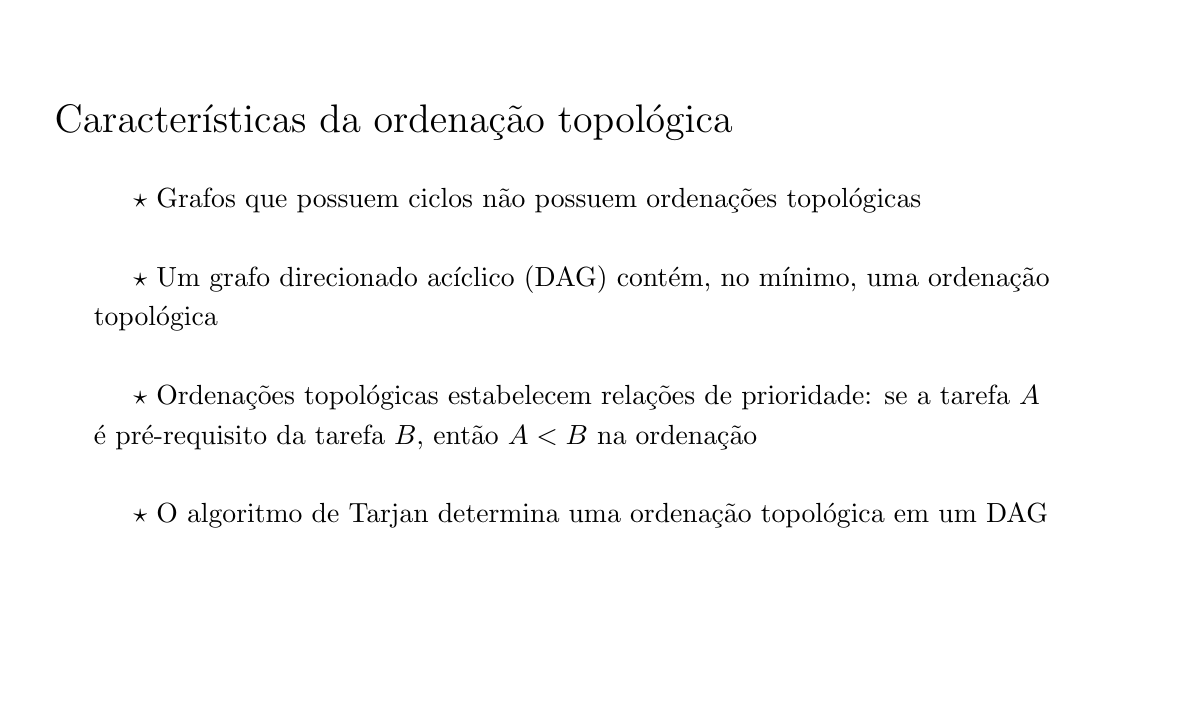
\begin{tikzpicture}
\node[draw,opacity=0] at (0, 0) {x};
\node[draw,opacity=0] at (14, 8) {x};

	\node[anchor=west] (title) at (0.0, 7.0) { \Large \bbbold{Características da ordenação topológica} };

	\node[anchor=west] (a) at (1.0, 6.0) { $\star$ \bbtext{Grafos que possuem ciclos não possuem ordenações topológicas} };


	\node[anchor=west] (b) at (1.0, 5.0) { $\star$ \bbtext{Um grafo direcionado acíclico (DAG) contém, no mínimo, uma ordenação } };

	\node[anchor=west] (b1) at (0.5, 4.5) { \bbtext{topológica} };


	\node[anchor=west] (c) at (1.0, 3.5) { $\star$ \bbtext{Ordenações topológicas estabelecem relações de prioridade: se a tarefa $A$} };

	\node[anchor=west] (c1) at (0.5, 3.0) { \bbtext{é pré-requisito da tarefa $B$, então $A < B$ na ordenação} };


	\node[anchor=west] (d) at (1.0, 2.0) { $\star$ \bbtext{O algoritmo de Tarjan determina uma ordenação topológica em um DAG} };

\end{tikzpicture}
\end{frame}
\begin{frame}[plain,t]
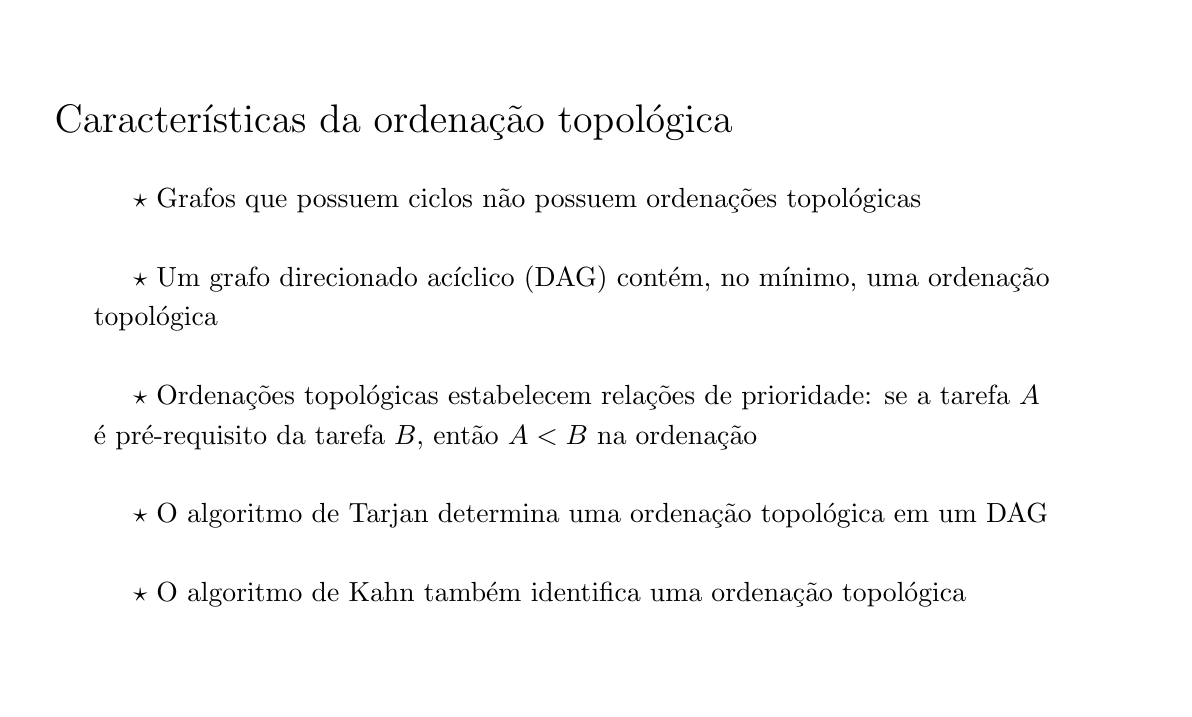
\begin{tikzpicture}
\node[draw,opacity=0] at (0, 0) {x};
\node[draw,opacity=0] at (14, 8) {x};

	\node[anchor=west] (title) at (0.0, 7.0) { \Large \bbbold{Características da ordenação topológica} };

	\node[anchor=west] (a) at (1.0, 6.0) { $\star$ \bbtext{Grafos que possuem ciclos não possuem ordenações topológicas} };


	\node[anchor=west] (b) at (1.0, 5.0) { $\star$ \bbtext{Um grafo direcionado acíclico (DAG) contém, no mínimo, uma ordenação } };

	\node[anchor=west] (b1) at (0.5, 4.5) { \bbtext{topológica} };


	\node[anchor=west] (c) at (1.0, 3.5) { $\star$ \bbtext{Ordenações topológicas estabelecem relações de prioridade: se a tarefa $A$} };

	\node[anchor=west] (c1) at (0.5, 3.0) { \bbtext{é pré-requisito da tarefa $B$, então $A < B$ na ordenação} };


	\node[anchor=west] (d) at (1.0, 2.0) { $\star$ \bbtext{O algoritmo de Tarjan determina uma ordenação topológica em um DAG} };


	\node[anchor=west] (e) at (1.0, 1.0) { $\star$ \bbtext{O algoritmo de Kahn também identifica uma ordenação topológica } };

\end{tikzpicture}
\end{frame}
\begin{frame}[plain,t]
\begin{tikzpicture}
\node[draw,opacity=0] at (0, 0) {x};
\node[draw,opacity=0] at (14, 8) {x};

	\node[anchor=west] (title) at (0.0, 7.0) { \Large \bbbold{Proponente do algoritmo de Tarjan} };

	\node[] (tarjan) at (7.0, 4.0) { \includegraphics[scale=0.12]{figs/tarjan.jpg} };

	\node[] (tname) at (7.0, 1.0) { \bbbold{Robert Endre Tarjan} };

	\node[] (tdate) at (7.0, 0.5) { \bbtext{(1976)} };

\end{tikzpicture}
\end{frame}
\begin{frame}[plain,t]
\begin{tikzpicture}
\node[draw,opacity=0] at (0, 0) {x};
\node[draw,opacity=0] at (14, 8) {x};

	\node[anchor=west] (title) at (0.0, 7.0) { \Large \bbbold{Características do algoritmo de Tarjan} };
\end{tikzpicture}
\end{frame}
\begin{frame}[plain,t]
\begin{tikzpicture}
\node[draw,opacity=0] at (0, 0) {x};
\node[draw,opacity=0] at (14, 8) {x};

	\node[anchor=west] (title) at (0.0, 7.0) { \Large \bbbold{Características do algoritmo de Tarjan} };

	\node[anchor=west] (a) at (1.0, 6.0) { $\star$ \bbtext{O algoritmo de Tarjan determina uma ordenação topológica em um DAG} };

	\node[anchor=west] (a1) at (0.5, 5.5) { \bbtext{por meio de uma DFS modificada} };

\end{tikzpicture}
\end{frame}
\begin{frame}[plain,t]
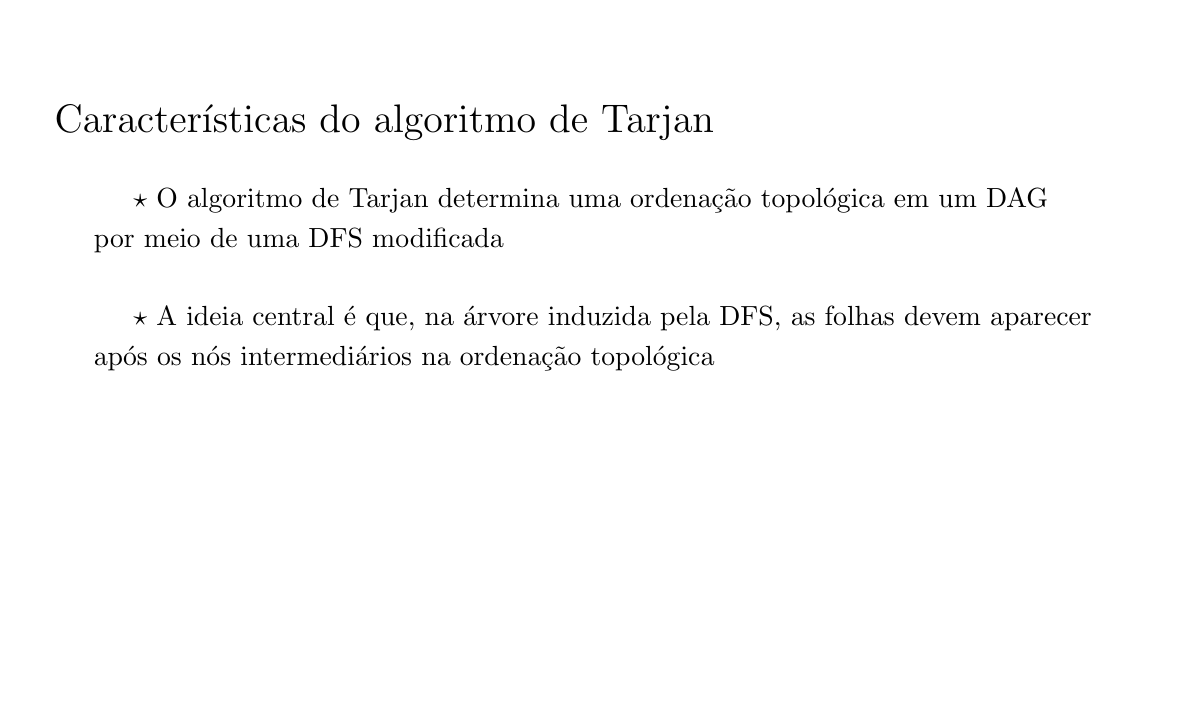
\begin{tikzpicture}
\node[draw,opacity=0] at (0, 0) {x};
\node[draw,opacity=0] at (14, 8) {x};

	\node[anchor=west] (title) at (0.0, 7.0) { \Large \bbbold{Características do algoritmo de Tarjan} };

	\node[anchor=west] (a) at (1.0, 6.0) { $\star$ \bbtext{O algoritmo de Tarjan determina uma ordenação topológica em um DAG} };

	\node[anchor=west] (a1) at (0.5, 5.5) { \bbtext{por meio de uma DFS modificada} };


	\node[anchor=west] (b) at (1.0, 4.5) { $\star$ \bbtext{A ideia central é que, na árvore induzida pela DFS, as folhas devem aparecer} };

	\node[anchor=west] (b1) at (0.5, 4.0) { \bbtext{após os nós intermediários na ordenação topológica} };

\end{tikzpicture}
\end{frame}
\begin{frame}[plain,t]
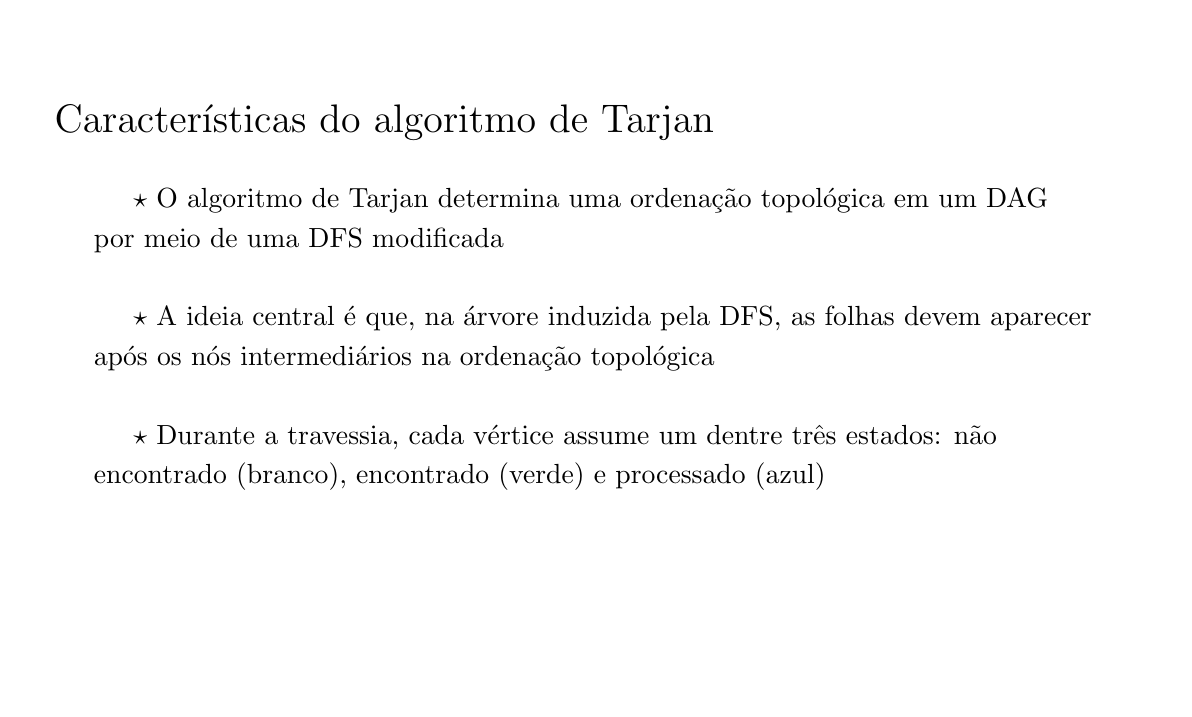
\begin{tikzpicture}
\node[draw,opacity=0] at (0, 0) {x};
\node[draw,opacity=0] at (14, 8) {x};

	\node[anchor=west] (title) at (0.0, 7.0) { \Large \bbbold{Características do algoritmo de Tarjan} };

	\node[anchor=west] (a) at (1.0, 6.0) { $\star$ \bbtext{O algoritmo de Tarjan determina uma ordenação topológica em um DAG} };

	\node[anchor=west] (a1) at (0.5, 5.5) { \bbtext{por meio de uma DFS modificada} };


	\node[anchor=west] (b) at (1.0, 4.5) { $\star$ \bbtext{A ideia central é que, na árvore induzida pela DFS, as folhas devem aparecer} };

	\node[anchor=west] (b1) at (0.5, 4.0) { \bbtext{após os nós intermediários na ordenação topológica} };


	\node[anchor=west] (c) at (1.0, 3.0) { $\star$ \bbtext{Durante a travessia, cada vértice assume um dentre três estados: não} };

	\node[anchor=west] (c1) at (0.5, 2.5) { \bbtext{encontrado (branco), encontrado (verde) e processado (azul)} };

\end{tikzpicture}
\end{frame}
\begin{frame}[plain,t]
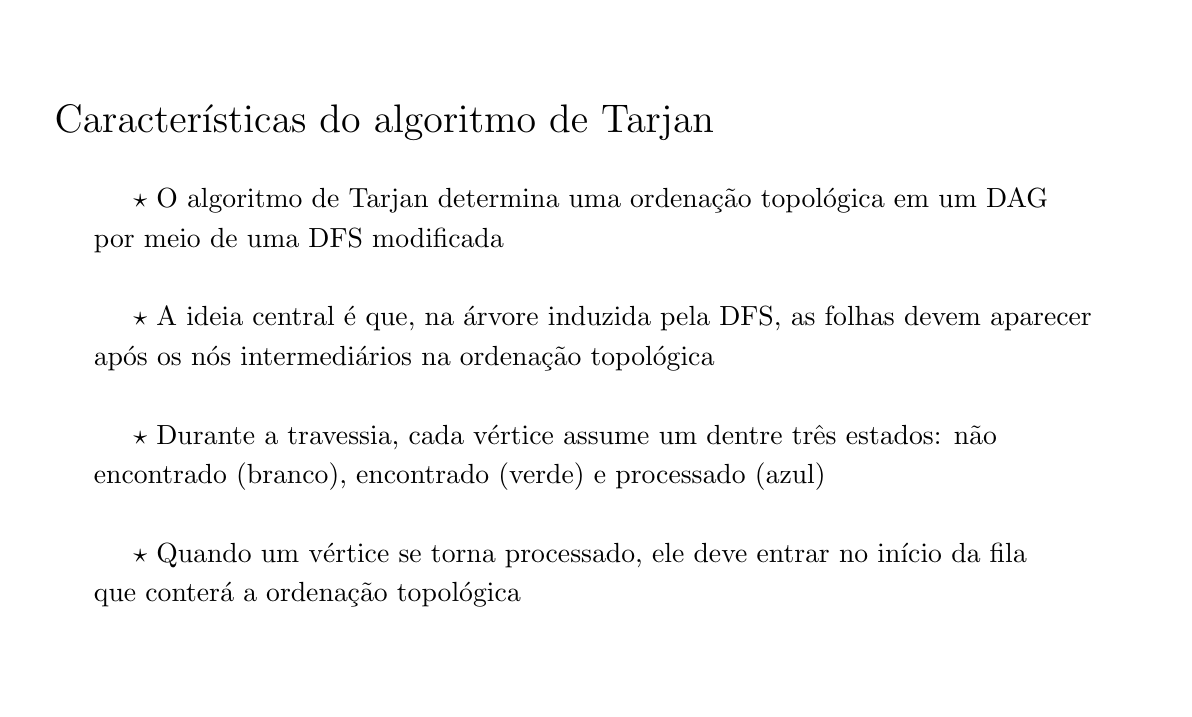
\begin{tikzpicture}
\node[draw,opacity=0] at (0, 0) {x};
\node[draw,opacity=0] at (14, 8) {x};

	\node[anchor=west] (title) at (0.0, 7.0) { \Large \bbbold{Características do algoritmo de Tarjan} };

	\node[anchor=west] (a) at (1.0, 6.0) { $\star$ \bbtext{O algoritmo de Tarjan determina uma ordenação topológica em um DAG} };

	\node[anchor=west] (a1) at (0.5, 5.5) { \bbtext{por meio de uma DFS modificada} };


	\node[anchor=west] (b) at (1.0, 4.5) { $\star$ \bbtext{A ideia central é que, na árvore induzida pela DFS, as folhas devem aparecer} };

	\node[anchor=west] (b1) at (0.5, 4.0) { \bbtext{após os nós intermediários na ordenação topológica} };


	\node[anchor=west] (c) at (1.0, 3.0) { $\star$ \bbtext{Durante a travessia, cada vértice assume um dentre três estados: não} };

	\node[anchor=west] (c1) at (0.5, 2.5) { \bbtext{encontrado (branco), encontrado (verde) e processado (azul)} };


	\node[anchor=west] (d) at (1.0, 1.5) { $\star$ \bbtext{Quando um vértice se torna processado, ele deve entrar no início da fila} };

	\node[anchor=west] (d1) at (0.5, 1.0) { \bbtext{que conterá a ordenação topológica} };

\end{tikzpicture}
\end{frame}
\begin{frame}[plain,t]
\begin{tikzpicture}
\node[draw,opacity=0] at (0, 0) {x};
\node[draw,opacity=0] at (14, 8) {x};

	\node[anchor=west] (title) at (0.0, 7.0) { \Large \bbbold{Pseudocódigo} };

\end{tikzpicture}
\end{frame}
\begin{frame}[plain,t]
\begin{tikzpicture}
\node[draw,opacity=0] at (0, 0) {x};
\node[draw,opacity=0] at (14, 8) {x};

	\node[anchor=west] (title) at (0.0, 7.0) { \Large \bbbold{Pseudocódigo} };


	\node[anchor=west] (input) at (0.5, 6.0) { \bbemph{Entrada:} \bbtext{um grafo direcionado acíclico $G(V, E)$} };

	\node[anchor=west] (output) at (0.5, 5.5) { \bbemph{Saída:} \bbtext{uma ordenação topológica $O$ de $G$} };

\end{tikzpicture}
\end{frame}
\begin{frame}[plain,t]
\begin{tikzpicture}
\node[draw,opacity=0] at (0, 0) {x};
\node[draw,opacity=0] at (14, 8) {x};

	\node[anchor=west] (title) at (0.0, 7.0) { \Large \bbbold{Pseudocódigo} };


	\node[anchor=west] (input) at (0.5, 6.0) { \bbemph{Entrada:} \bbtext{um grafo direcionado acíclico $G(V, E)$} };

	\node[anchor=west] (output) at (0.5, 5.5) { \bbemph{Saída:} \bbtext{uma ordenação topológica $O$ de $G$} };


	\node[anchor=west] (step1) at (1.0, 4.5) { $1.$ \bbtext{Marque todos os vértices $v\in V$ como não encontrados} };

\end{tikzpicture}
\end{frame}
\begin{frame}[plain,t]
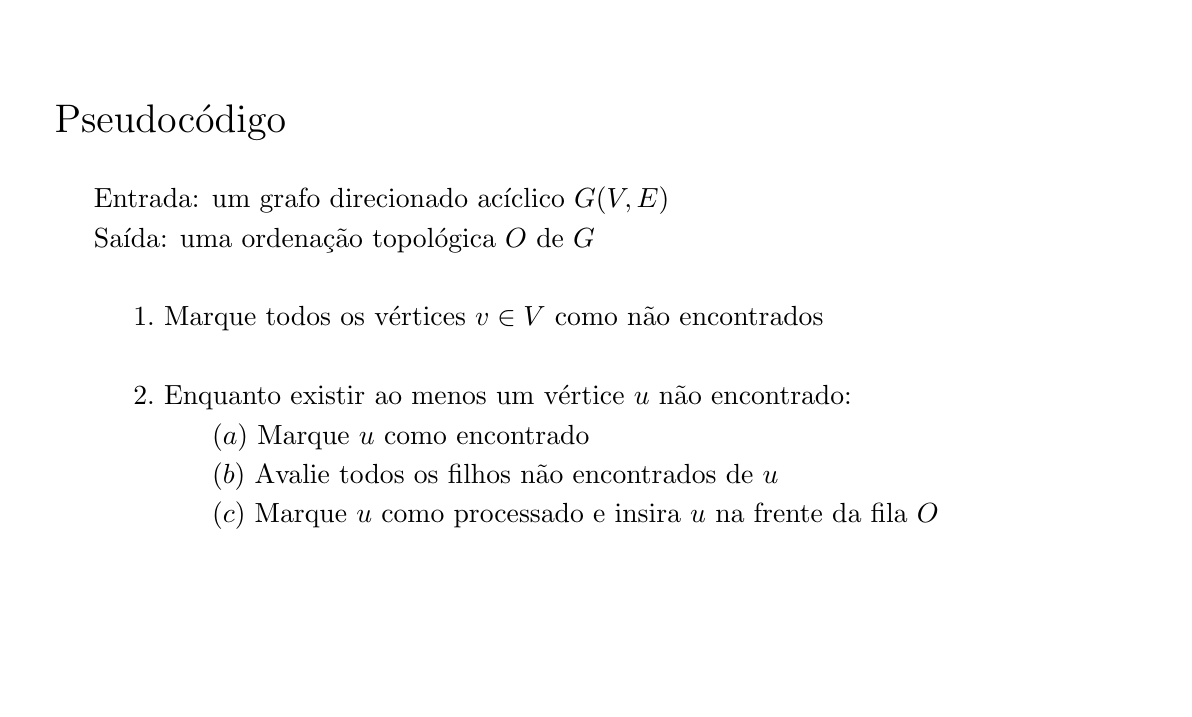
\begin{tikzpicture}
\node[draw,opacity=0] at (0, 0) {x};
\node[draw,opacity=0] at (14, 8) {x};

	\node[anchor=west] (title) at (0.0, 7.0) { \Large \bbbold{Pseudocódigo} };


	\node[anchor=west] (input) at (0.5, 6.0) { \bbemph{Entrada:} \bbtext{um grafo direcionado acíclico $G(V, E)$} };

	\node[anchor=west] (output) at (0.5, 5.5) { \bbemph{Saída:} \bbtext{uma ordenação topológica $O$ de $G$} };


	\node[anchor=west] (step1) at (1.0, 4.5) { $1.$ \bbtext{Marque todos os vértices $v\in V$ como não encontrados} };


	\node[anchor=west] (step2) at (1.0, 3.5) { $2.$ \bbtext{Enquanto existir ao menos um vértice $u$ não encontrado:} };

	\node[anchor=west] (step2a) at (2.0, 3.0) { $(a)$ \bbtext{Marque $u$ como encontrado} };

	\node[anchor=west] (step2b) at (2.0, 2.5) { $(b)$ \bbtext{Avalie todos os filhos não encontrados de $u$} };

	\node[anchor=west] (step2c) at (2.0, 2.0) { $(c)$ \bbtext{Marque $u$ como processado e insira $u$ na frente da fila $O$} };

\end{tikzpicture}
\end{frame}
\begin{frame}[plain,t]
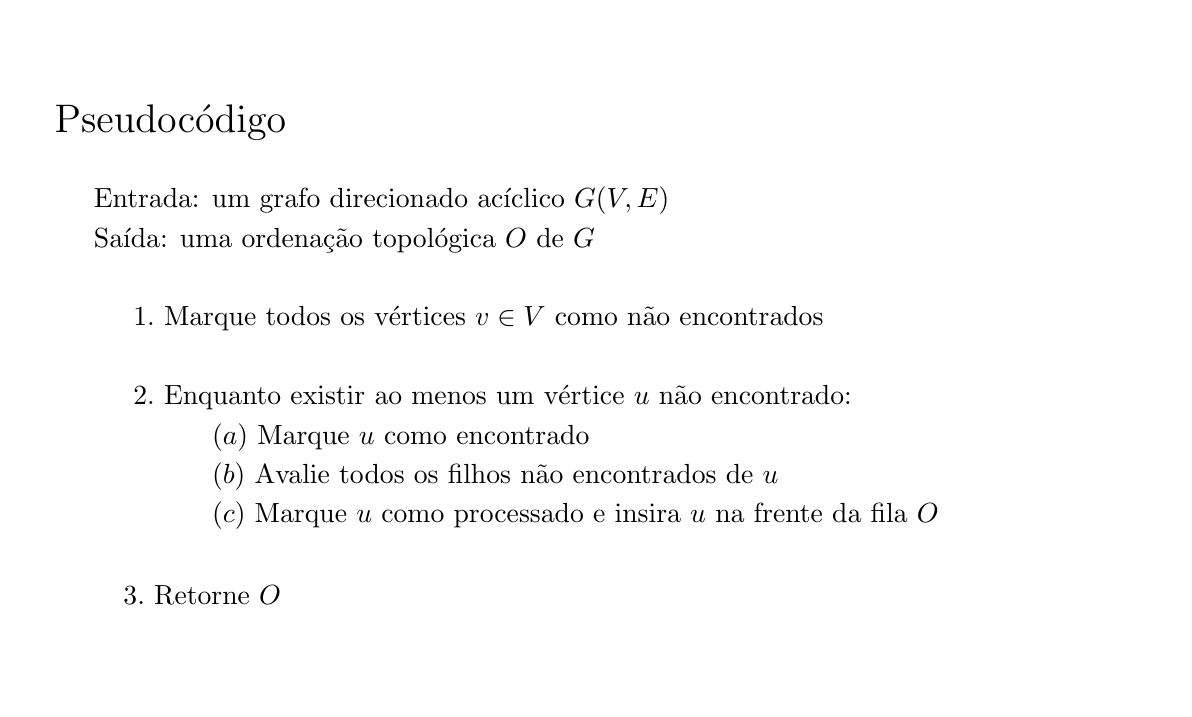
\begin{tikzpicture}
\node[draw,opacity=0] at (0, 0) {x};
\node[draw,opacity=0] at (14, 8) {x};

	\node[anchor=west] (title) at (0.0, 7.0) { \Large \bbbold{Pseudocódigo} };


	\node[anchor=west] (input) at (0.5, 6.0) { \bbemph{Entrada:} \bbtext{um grafo direcionado acíclico $G(V, E)$} };

	\node[anchor=west] (output) at (0.5, 5.5) { \bbemph{Saída:} \bbtext{uma ordenação topológica $O$ de $G$} };


	\node[anchor=west] (step1) at (1.0, 4.5) { $1.$ \bbtext{Marque todos os vértices $v\in V$ como não encontrados} };


	\node[anchor=west] (step2) at (1.0, 3.5) { $2.$ \bbtext{Enquanto existir ao menos um vértice $u$ não encontrado:} };

	\node[anchor=west] (step2a) at (2.0, 3.0) { $(a)$ \bbtext{Marque $u$ como encontrado} };

	\node[anchor=west] (step2b) at (2.0, 2.5) { $(b)$ \bbtext{Avalie todos os filhos não encontrados de $u$} };

	\node[anchor=west] (step2c) at (2.0, 2.0) { $(c)$ \bbtext{Marque $u$ como processado e insira $u$ na frente da fila $O$} };


	\node[] (step3) at (2.0, 1.0) { $3.$ \bbtext{Retorne $O$} };

\end{tikzpicture}
\end{frame}
\begin{frame}[plain,t]
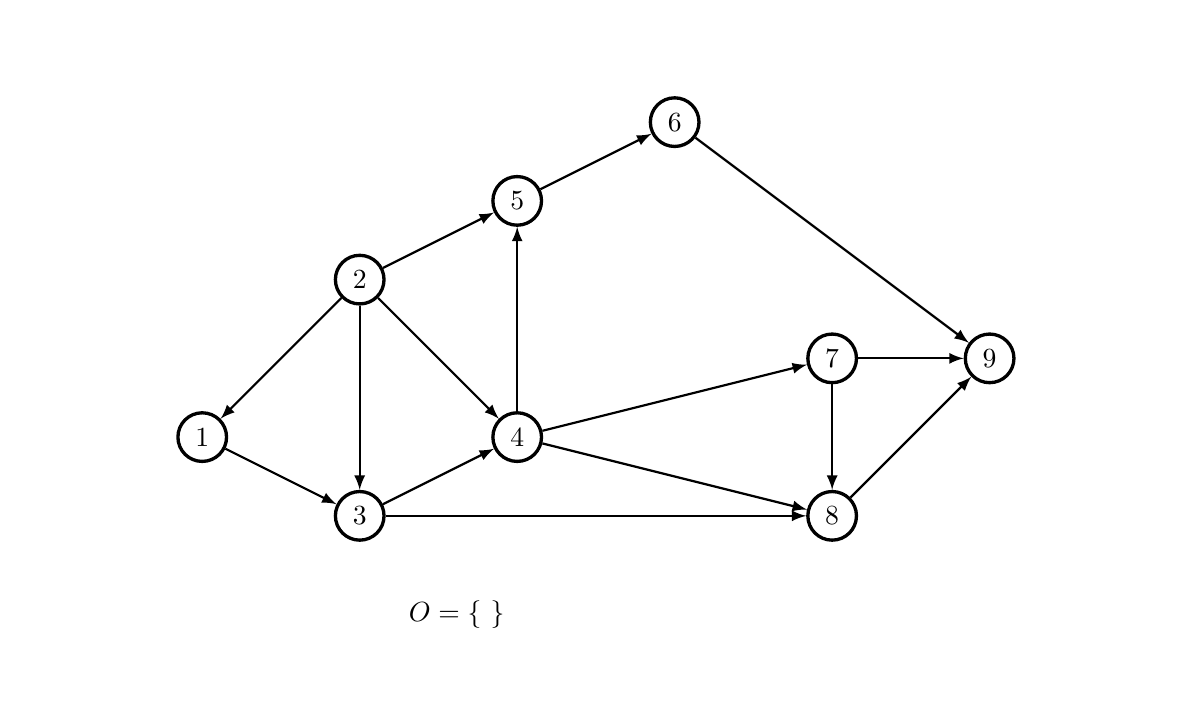
\begin{tikzpicture}
\node[draw,opacity=0] at (0, 0) {x};
\node[draw,opacity=0] at (14, 8) {x};

	\node[very thick,draw,circle] (node1) at (2.0, 3.0) { \bbtext{1} };

	\node[very thick,draw,circle] (node2) at (4.0, 5.0) { \bbtext{2} };

	\node[very thick,draw,circle] (node3) at (4.0, 2.0) { \bbtext{3} };

	\node[very thick,draw,circle] (node4) at (6.0, 3.0) { \bbtext{4} };

	\node[very thick,draw,circle] (node5) at (6.0, 6.0) { \bbtext{5} };

	\node[very thick,draw,circle] (node6) at (8.0, 7.0) { \bbtext{6} };

	\node[very thick,draw,circle] (node7) at (10.0, 4.0) { \bbtext{7} };

	\node[very thick,draw,circle] (node8) at (10.0, 2.0) { \bbtext{8} };

	\node[very thick,draw,circle] (node9) at (12.0, 4.0) { \bbtext{9} };


	\node[anchor=west] (O) at (4.5, 0.75) { \bbtext{$O = \{\ \}$} };

	\draw[thick,-latex](node2) to (node1);

	\draw[thick,-latex](node2) to (node3);

	\draw[thick,-latex](node2) to (node4);

	\draw[thick,-latex](node2) to (node5);

	\draw[thick,-latex](node1) to (node3);

	\draw[thick,-latex](node3) to (node4);

	\draw[thick,-latex](node3) to (node8);

	\draw[thick,-latex](node4) to (node5);

	\draw[thick,-latex](node4) to (node7);

	\draw[thick,-latex](node4) to (node8);

	\draw[thick,-latex](node5) to (node6);

	\draw[thick,-latex](node6) to (node9);

	\draw[thick,-latex](node7) to (node8);

	\draw[thick,-latex](node7) to (node9);

	\draw[thick,-latex](node8) to (node9);

\end{tikzpicture}
\end{frame}
\begin{frame}[plain,t]
\begin{tikzpicture}
\node[draw,opacity=0] at (0, 0) {x};
\node[draw,opacity=0] at (14, 8) {x};

	\node[very thick,draw,circle,fill=BBGreen] (node1) at (2.0, 3.0) { \bbtext{1} };

	\node[very thick,draw,circle] (node2) at (4.0, 5.0) { \bbtext{2} };

	\node[very thick,draw,circle] (node3) at (4.0, 2.0) { \bbtext{3} };

	\node[very thick,draw,circle] (node4) at (6.0, 3.0) { \bbtext{4} };

	\node[very thick,draw,circle] (node5) at (6.0, 6.0) { \bbtext{5} };

	\node[very thick,draw,circle] (node6) at (8.0, 7.0) { \bbtext{6} };

	\node[very thick,draw,circle] (node7) at (10.0, 4.0) { \bbtext{7} };

	\node[very thick,draw,circle] (node8) at (10.0, 2.0) { \bbtext{8} };

	\node[very thick,draw,circle] (node9) at (12.0, 4.0) { \bbtext{9} };


	\node[anchor=west] (O) at (4.5, 0.75) { \bbtext{$O = \{\ \}$} };

	\draw[thick,-latex](node2) to (node1);

	\draw[thick,-latex](node2) to (node3);

	\draw[thick,-latex](node2) to (node4);

	\draw[thick,-latex](node2) to (node5);

	\draw[thick,-latex](node1) to (node3);

	\draw[thick,-latex](node3) to (node4);

	\draw[thick,-latex](node3) to (node8);

	\draw[thick,-latex](node4) to (node5);

	\draw[thick,-latex](node4) to (node7);

	\draw[thick,-latex](node4) to (node8);

	\draw[thick,-latex](node5) to (node6);

	\draw[thick,-latex](node6) to (node9);

	\draw[thick,-latex](node7) to (node8);

	\draw[thick,-latex](node7) to (node9);

	\draw[thick,-latex](node8) to (node9);



\end{tikzpicture}
\end{frame}
\begin{frame}[plain,t]
\begin{tikzpicture}
\node[draw,opacity=0] at (0, 0) {x};
\node[draw,opacity=0] at (14, 8) {x};

	\node[very thick,draw,circle,fill=BBGreen] (node1) at (2.0, 3.0) { \bbtext{1} };

	\node[very thick,draw,circle] (node2) at (4.0, 5.0) { \bbtext{2} };

	\node[very thick,draw,circle,fill=BBGreen] (node3) at (4.0, 2.0) { \bbtext{3} };

	\node[very thick,draw,circle] (node4) at (6.0, 3.0) { \bbtext{4} };

	\node[very thick,draw,circle] (node5) at (6.0, 6.0) { \bbtext{5} };

	\node[very thick,draw,circle] (node6) at (8.0, 7.0) { \bbtext{6} };

	\node[very thick,draw,circle] (node7) at (10.0, 4.0) { \bbtext{7} };

	\node[very thick,draw,circle] (node8) at (10.0, 2.0) { \bbtext{8} };

	\node[very thick,draw,circle] (node9) at (12.0, 4.0) { \bbtext{9} };


	\node[anchor=west] (O) at (4.5, 0.75) { \bbtext{$O = \{\ \}$} };

	\draw[thick,-latex](node2) to (node1);

	\draw[thick,-latex](node2) to (node3);

	\draw[thick,-latex](node2) to (node4);

	\draw[thick,-latex](node2) to (node5);

	\draw[thick,-latex](node1) to (node3);

	\draw[thick,-latex](node3) to (node4);

	\draw[thick,-latex](node3) to (node8);

	\draw[thick,-latex](node4) to (node5);

	\draw[thick,-latex](node4) to (node7);

	\draw[thick,-latex](node4) to (node8);

	\draw[thick,-latex](node5) to (node6);

	\draw[thick,-latex](node6) to (node9);

	\draw[thick,-latex](node7) to (node8);

	\draw[thick,-latex](node7) to (node9);

	\draw[thick,-latex](node8) to (node9);





\end{tikzpicture}
\end{frame}
\begin{frame}[plain,t]
\begin{tikzpicture}
\node[draw,opacity=0] at (0, 0) {x};
\node[draw,opacity=0] at (14, 8) {x};

	\node[very thick,draw,circle,fill=BBGreen] (node1) at (2.0, 3.0) { \bbtext{1} };

	\node[very thick,draw,circle] (node2) at (4.0, 5.0) { \bbtext{2} };

	\node[very thick,draw,circle,fill=BBGreen] (node3) at (4.0, 2.0) { \bbtext{3} };

	\node[very thick,draw,circle,fill=BBGreen] (node4) at (6.0, 3.0) { \bbtext{4} };

	\node[very thick,draw,circle] (node5) at (6.0, 6.0) { \bbtext{5} };

	\node[very thick,draw,circle] (node6) at (8.0, 7.0) { \bbtext{6} };

	\node[very thick,draw,circle] (node7) at (10.0, 4.0) { \bbtext{7} };

	\node[very thick,draw,circle] (node8) at (10.0, 2.0) { \bbtext{8} };

	\node[very thick,draw,circle] (node9) at (12.0, 4.0) { \bbtext{9} };


	\node[anchor=west] (O) at (4.5, 0.75) { \bbtext{$O = \{\ \}$} };

	\draw[thick,-latex](node2) to (node1);

	\draw[thick,-latex](node2) to (node3);

	\draw[thick,-latex](node2) to (node4);

	\draw[thick,-latex](node2) to (node5);

	\draw[thick,-latex](node1) to (node3);

	\draw[thick,-latex](node3) to (node4);

	\draw[thick,-latex](node3) to (node8);

	\draw[thick,-latex](node4) to (node5);

	\draw[thick,-latex](node4) to (node7);

	\draw[thick,-latex](node4) to (node8);

	\draw[thick,-latex](node5) to (node6);

	\draw[thick,-latex](node6) to (node9);

	\draw[thick,-latex](node7) to (node8);

	\draw[thick,-latex](node7) to (node9);

	\draw[thick,-latex](node8) to (node9);







\end{tikzpicture}
\end{frame}
\begin{frame}[plain,t]
\begin{tikzpicture}
\node[draw,opacity=0] at (0, 0) {x};
\node[draw,opacity=0] at (14, 8) {x};

	\node[very thick,draw,circle,fill=BBGreen] (node1) at (2.0, 3.0) { \bbtext{1} };

	\node[very thick,draw,circle] (node2) at (4.0, 5.0) { \bbtext{2} };

	\node[very thick,draw,circle,fill=BBGreen] (node3) at (4.0, 2.0) { \bbtext{3} };

	\node[very thick,draw,circle,fill=BBGreen] (node4) at (6.0, 3.0) { \bbtext{4} };

	\node[very thick,draw,circle,fill=BBGreen] (node5) at (6.0, 6.0) { \bbtext{5} };

	\node[very thick,draw,circle] (node6) at (8.0, 7.0) { \bbtext{6} };

	\node[very thick,draw,circle] (node7) at (10.0, 4.0) { \bbtext{7} };

	\node[very thick,draw,circle] (node8) at (10.0, 2.0) { \bbtext{8} };

	\node[very thick,draw,circle] (node9) at (12.0, 4.0) { \bbtext{9} };


	\node[anchor=west] (O) at (4.5, 0.75) { \bbtext{$O = \{\ \}$} };

	\draw[thick,-latex](node2) to (node1);

	\draw[thick,-latex](node2) to (node3);

	\draw[thick,-latex](node2) to (node4);

	\draw[thick,-latex](node2) to (node5);

	\draw[thick,-latex](node1) to (node3);

	\draw[thick,-latex](node3) to (node4);

	\draw[thick,-latex](node3) to (node8);

	\draw[thick,-latex](node4) to (node5);

	\draw[thick,-latex](node4) to (node7);

	\draw[thick,-latex](node4) to (node8);

	\draw[thick,-latex](node5) to (node6);

	\draw[thick,-latex](node6) to (node9);

	\draw[thick,-latex](node7) to (node8);

	\draw[thick,-latex](node7) to (node9);

	\draw[thick,-latex](node8) to (node9);









\end{tikzpicture}
\end{frame}
\begin{frame}[plain,t]
\begin{tikzpicture}
\node[draw,opacity=0] at (0, 0) {x};
\node[draw,opacity=0] at (14, 8) {x};

	\node[very thick,draw,circle,fill=BBGreen] (node1) at (2.0, 3.0) { \bbtext{1} };

	\node[very thick,draw,circle] (node2) at (4.0, 5.0) { \bbtext{2} };

	\node[very thick,draw,circle,fill=BBGreen] (node3) at (4.0, 2.0) { \bbtext{3} };

	\node[very thick,draw,circle,fill=BBGreen] (node4) at (6.0, 3.0) { \bbtext{4} };

	\node[very thick,draw,circle,fill=BBGreen] (node5) at (6.0, 6.0) { \bbtext{5} };

	\node[very thick,draw,circle,fill=BBGreen] (node6) at (8.0, 7.0) { \bbtext{6} };

	\node[very thick,draw,circle] (node7) at (10.0, 4.0) { \bbtext{7} };

	\node[very thick,draw,circle] (node8) at (10.0, 2.0) { \bbtext{8} };

	\node[very thick,draw,circle] (node9) at (12.0, 4.0) { \bbtext{9} };


	\node[anchor=west] (O) at (4.5, 0.75) { \bbtext{$O = \{\ \}$} };

	\draw[thick,-latex](node2) to (node1);

	\draw[thick,-latex](node2) to (node3);

	\draw[thick,-latex](node2) to (node4);

	\draw[thick,-latex](node2) to (node5);

	\draw[thick,-latex](node1) to (node3);

	\draw[thick,-latex](node3) to (node4);

	\draw[thick,-latex](node3) to (node8);

	\draw[thick,-latex](node4) to (node5);

	\draw[thick,-latex](node4) to (node7);

	\draw[thick,-latex](node4) to (node8);

	\draw[thick,-latex](node5) to (node6);

	\draw[thick,-latex](node6) to (node9);

	\draw[thick,-latex](node7) to (node8);

	\draw[thick,-latex](node7) to (node9);

	\draw[thick,-latex](node8) to (node9);











\end{tikzpicture}
\end{frame}
\begin{frame}[plain,t]
\begin{tikzpicture}
\node[draw,opacity=0] at (0, 0) {x};
\node[draw,opacity=0] at (14, 8) {x};

	\node[very thick,draw,circle,fill=BBGreen] (node1) at (2.0, 3.0) { \bbtext{1} };

	\node[very thick,draw,circle] (node2) at (4.0, 5.0) { \bbtext{2} };

	\node[very thick,draw,circle,fill=BBGreen] (node3) at (4.0, 2.0) { \bbtext{3} };

	\node[very thick,draw,circle,fill=BBGreen] (node4) at (6.0, 3.0) { \bbtext{4} };

	\node[very thick,draw,circle,fill=BBGreen] (node5) at (6.0, 6.0) { \bbtext{5} };

	\node[very thick,draw,circle,fill=BBGreen] (node6) at (8.0, 7.0) { \bbtext{6} };

	\node[very thick,draw,circle] (node7) at (10.0, 4.0) { \bbtext{7} };

	\node[very thick,draw,circle] (node8) at (10.0, 2.0) { \bbtext{8} };

	\node[very thick,draw,circle,fill=BBGreen] (node9) at (12.0, 4.0) { \bbtext{9} };


	\node[anchor=west] (O) at (4.5, 0.75) { \bbtext{$O = \{\ \}$} };

	\draw[thick,-latex](node2) to (node1);

	\draw[thick,-latex](node2) to (node3);

	\draw[thick,-latex](node2) to (node4);

	\draw[thick,-latex](node2) to (node5);

	\draw[thick,-latex](node1) to (node3);

	\draw[thick,-latex](node3) to (node4);

	\draw[thick,-latex](node3) to (node8);

	\draw[thick,-latex](node4) to (node5);

	\draw[thick,-latex](node4) to (node7);

	\draw[thick,-latex](node4) to (node8);

	\draw[thick,-latex](node5) to (node6);

	\draw[thick,-latex](node6) to (node9);

	\draw[thick,-latex](node7) to (node8);

	\draw[thick,-latex](node7) to (node9);

	\draw[thick,-latex](node8) to (node9);













\end{tikzpicture}
\end{frame}
\begin{frame}[plain,t]
\begin{tikzpicture}
\node[draw,opacity=0] at (0, 0) {x};
\node[draw,opacity=0] at (14, 8) {x};

	\node[very thick,draw,circle,fill=BBGreen] (node1) at (2.0, 3.0) { \bbtext{1} };

	\node[very thick,draw,circle] (node2) at (4.0, 5.0) { \bbtext{2} };

	\node[very thick,draw,circle,fill=BBGreen] (node3) at (4.0, 2.0) { \bbtext{3} };

	\node[very thick,draw,circle,fill=BBGreen] (node4) at (6.0, 3.0) { \bbtext{4} };

	\node[very thick,draw,circle,fill=BBGreen] (node5) at (6.0, 6.0) { \bbtext{5} };

	\node[very thick,draw,circle,fill=BBGreen] (node6) at (8.0, 7.0) { \bbtext{6} };

	\node[very thick,draw,circle] (node7) at (10.0, 4.0) { \bbtext{7} };

	\node[very thick,draw,circle] (node8) at (10.0, 2.0) { \bbtext{8} };

	\node[very thick,draw,circle,fill=BBCyan] (node9) at (12.0, 4.0) { \bbtext{9} };


	\node[anchor=west] (O) at (4.5, 0.75) { \bbtext{$O = \{$ 9 $\}$} };

	\draw[thick,-latex](node2) to (node1);

	\draw[thick,-latex](node2) to (node3);

	\draw[thick,-latex](node2) to (node4);

	\draw[thick,-latex](node2) to (node5);

	\draw[thick,-latex](node1) to (node3);

	\draw[thick,-latex](node3) to (node4);

	\draw[thick,-latex](node3) to (node8);

	\draw[thick,-latex](node4) to (node5);

	\draw[thick,-latex](node4) to (node7);

	\draw[thick,-latex](node4) to (node8);

	\draw[thick,-latex](node5) to (node6);

	\draw[thick,-latex](node6) to (node9);

	\draw[thick,-latex](node7) to (node8);

	\draw[thick,-latex](node7) to (node9);

	\draw[thick,-latex](node8) to (node9);















\end{tikzpicture}
\end{frame}
\begin{frame}[plain,t]
\begin{tikzpicture}
\node[draw,opacity=0] at (0, 0) {x};
\node[draw,opacity=0] at (14, 8) {x};

	\node[very thick,draw,circle,fill=BBGreen] (node1) at (2.0, 3.0) { \bbtext{1} };

	\node[very thick,draw,circle] (node2) at (4.0, 5.0) { \bbtext{2} };

	\node[very thick,draw,circle,fill=BBGreen] (node3) at (4.0, 2.0) { \bbtext{3} };

	\node[very thick,draw,circle,fill=BBGreen] (node4) at (6.0, 3.0) { \bbtext{4} };

	\node[very thick,draw,circle,fill=BBGreen] (node5) at (6.0, 6.0) { \bbtext{5} };

	\node[very thick,draw,circle,fill=BBCyan] (node6) at (8.0, 7.0) { \bbtext{6} };

	\node[very thick,draw,circle] (node7) at (10.0, 4.0) { \bbtext{7} };

	\node[very thick,draw,circle] (node8) at (10.0, 2.0) { \bbtext{8} };

	\node[very thick,draw,circle,fill=BBCyan] (node9) at (12.0, 4.0) { \bbtext{9} };


	\node[anchor=west] (O) at (4.5, 0.75) { \bbtext{$O = \{$ 6, 9 $\}$} };

	\draw[thick,-latex](node2) to (node1);

	\draw[thick,-latex](node2) to (node3);

	\draw[thick,-latex](node2) to (node4);

	\draw[thick,-latex](node2) to (node5);

	\draw[thick,-latex](node1) to (node3);

	\draw[thick,-latex](node3) to (node4);

	\draw[thick,-latex](node3) to (node8);

	\draw[thick,-latex](node4) to (node5);

	\draw[thick,-latex](node4) to (node7);

	\draw[thick,-latex](node4) to (node8);

	\draw[thick,-latex](node5) to (node6);

	\draw[thick,-latex](node6) to (node9);

	\draw[thick,-latex](node7) to (node8);

	\draw[thick,-latex](node7) to (node9);

	\draw[thick,-latex](node8) to (node9);

















\end{tikzpicture}
\end{frame}
\begin{frame}[plain,t]
\begin{tikzpicture}
\node[draw,opacity=0] at (0, 0) {x};
\node[draw,opacity=0] at (14, 8) {x};

	\node[very thick,draw,circle,fill=BBGreen] (node1) at (2.0, 3.0) { \bbtext{1} };

	\node[very thick,draw,circle] (node2) at (4.0, 5.0) { \bbtext{2} };

	\node[very thick,draw,circle,fill=BBGreen] (node3) at (4.0, 2.0) { \bbtext{3} };

	\node[very thick,draw,circle,fill=BBGreen] (node4) at (6.0, 3.0) { \bbtext{4} };

	\node[very thick,draw,circle,fill=BBCyan] (node5) at (6.0, 6.0) { \bbtext{5} };

	\node[very thick,draw,circle,fill=BBCyan] (node6) at (8.0, 7.0) { \bbtext{6} };

	\node[very thick,draw,circle] (node7) at (10.0, 4.0) { \bbtext{7} };

	\node[very thick,draw,circle] (node8) at (10.0, 2.0) { \bbtext{8} };

	\node[very thick,draw,circle,fill=BBCyan] (node9) at (12.0, 4.0) { \bbtext{9} };


	\node[anchor=west] (O) at (4.5, 0.75) { \bbtext{$O = \{$ 5, 6, 9 $\}$} };

	\draw[thick,-latex](node2) to (node1);

	\draw[thick,-latex](node2) to (node3);

	\draw[thick,-latex](node2) to (node4);

	\draw[thick,-latex](node2) to (node5);

	\draw[thick,-latex](node1) to (node3);

	\draw[thick,-latex](node3) to (node4);

	\draw[thick,-latex](node3) to (node8);

	\draw[thick,-latex](node4) to (node5);

	\draw[thick,-latex](node4) to (node7);

	\draw[thick,-latex](node4) to (node8);

	\draw[thick,-latex](node5) to (node6);

	\draw[thick,-latex](node6) to (node9);

	\draw[thick,-latex](node7) to (node8);

	\draw[thick,-latex](node7) to (node9);

	\draw[thick,-latex](node8) to (node9);



















\end{tikzpicture}
\end{frame}
\begin{frame}[plain,t]
\begin{tikzpicture}
\node[draw,opacity=0] at (0, 0) {x};
\node[draw,opacity=0] at (14, 8) {x};

	\node[very thick,draw,circle,fill=BBGreen] (node1) at (2.0, 3.0) { \bbtext{1} };

	\node[very thick,draw,circle] (node2) at (4.0, 5.0) { \bbtext{2} };

	\node[very thick,draw,circle,fill=BBGreen] (node3) at (4.0, 2.0) { \bbtext{3} };

	\node[very thick,draw,circle,fill=BBGreen] (node4) at (6.0, 3.0) { \bbtext{4} };

	\node[very thick,draw,circle,fill=BBCyan] (node5) at (6.0, 6.0) { \bbtext{5} };

	\node[very thick,draw,circle,fill=BBCyan] (node6) at (8.0, 7.0) { \bbtext{6} };

	\node[very thick,draw,circle,fill=BBGreen] (node7) at (10.0, 4.0) { \bbtext{7} };

	\node[very thick,draw,circle] (node8) at (10.0, 2.0) { \bbtext{8} };

	\node[very thick,draw,circle,fill=BBCyan] (node9) at (12.0, 4.0) { \bbtext{9} };


	\node[anchor=west] (O) at (4.5, 0.75) { \bbtext{$O = \{$ 5, 6, 9 $\}$} };

	\draw[thick,-latex](node2) to (node1);

	\draw[thick,-latex](node2) to (node3);

	\draw[thick,-latex](node2) to (node4);

	\draw[thick,-latex](node2) to (node5);

	\draw[thick,-latex](node1) to (node3);

	\draw[thick,-latex](node3) to (node4);

	\draw[thick,-latex](node3) to (node8);

	\draw[thick,-latex](node4) to (node5);

	\draw[thick,-latex](node4) to (node7);

	\draw[thick,-latex](node4) to (node8);

	\draw[thick,-latex](node5) to (node6);

	\draw[thick,-latex](node6) to (node9);

	\draw[thick,-latex](node7) to (node8);

	\draw[thick,-latex](node7) to (node9);

	\draw[thick,-latex](node8) to (node9);




















\end{tikzpicture}
\end{frame}
\begin{frame}[plain,t]
\begin{tikzpicture}
\node[draw,opacity=0] at (0, 0) {x};
\node[draw,opacity=0] at (14, 8) {x};

	\node[very thick,draw,circle,fill=BBGreen] (node1) at (2.0, 3.0) { \bbtext{1} };

	\node[very thick,draw,circle] (node2) at (4.0, 5.0) { \bbtext{2} };

	\node[very thick,draw,circle,fill=BBGreen] (node3) at (4.0, 2.0) { \bbtext{3} };

	\node[very thick,draw,circle,fill=BBGreen] (node4) at (6.0, 3.0) { \bbtext{4} };

	\node[very thick,draw,circle,fill=BBCyan] (node5) at (6.0, 6.0) { \bbtext{5} };

	\node[very thick,draw,circle,fill=BBCyan] (node6) at (8.0, 7.0) { \bbtext{6} };

	\node[very thick,draw,circle,fill=BBGreen] (node7) at (10.0, 4.0) { \bbtext{7} };

	\node[very thick,draw,circle,fill=BBGreen] (node8) at (10.0, 2.0) { \bbtext{8} };

	\node[very thick,draw,circle,fill=BBCyan] (node9) at (12.0, 4.0) { \bbtext{9} };


	\node[anchor=west] (O) at (4.5, 0.75) { \bbtext{$O = \{$ 5, 6, 9 $\}$} };

	\draw[thick,-latex](node2) to (node1);

	\draw[thick,-latex](node2) to (node3);

	\draw[thick,-latex](node2) to (node4);

	\draw[thick,-latex](node2) to (node5);

	\draw[thick,-latex](node1) to (node3);

	\draw[thick,-latex](node3) to (node4);

	\draw[thick,-latex](node3) to (node8);

	\draw[thick,-latex](node4) to (node5);

	\draw[thick,-latex](node4) to (node7);

	\draw[thick,-latex](node4) to (node8);

	\draw[thick,-latex](node5) to (node6);

	\draw[thick,-latex](node6) to (node9);

	\draw[thick,-latex](node7) to (node8);

	\draw[thick,-latex](node7) to (node9);

	\draw[thick,-latex](node8) to (node9);





















\end{tikzpicture}
\end{frame}
\begin{frame}[plain,t]
\begin{tikzpicture}
\node[draw,opacity=0] at (0, 0) {x};
\node[draw,opacity=0] at (14, 8) {x};

	\node[very thick,draw,circle,fill=BBGreen] (node1) at (2.0, 3.0) { \bbtext{1} };

	\node[very thick,draw,circle] (node2) at (4.0, 5.0) { \bbtext{2} };

	\node[very thick,draw,circle,fill=BBGreen] (node3) at (4.0, 2.0) { \bbtext{3} };

	\node[very thick,draw,circle,fill=BBGreen] (node4) at (6.0, 3.0) { \bbtext{4} };

	\node[very thick,draw,circle,fill=BBCyan] (node5) at (6.0, 6.0) { \bbtext{5} };

	\node[very thick,draw,circle,fill=BBCyan] (node6) at (8.0, 7.0) { \bbtext{6} };

	\node[very thick,draw,circle,fill=BBGreen] (node7) at (10.0, 4.0) { \bbtext{7} };

	\node[very thick,draw,circle,fill=BBCyan] (node8) at (10.0, 2.0) { \bbtext{8} };

	\node[very thick,draw,circle,fill=BBCyan] (node9) at (12.0, 4.0) { \bbtext{9} };


	\node[anchor=west] (O) at (4.5, 0.75) { \bbtext{$O = \{$ 8, 5, 6, 9 $\}$} };

	\draw[thick,-latex](node2) to (node1);

	\draw[thick,-latex](node2) to (node3);

	\draw[thick,-latex](node2) to (node4);

	\draw[thick,-latex](node2) to (node5);

	\draw[thick,-latex](node1) to (node3);

	\draw[thick,-latex](node3) to (node4);

	\draw[thick,-latex](node3) to (node8);

	\draw[thick,-latex](node4) to (node5);

	\draw[thick,-latex](node4) to (node7);

	\draw[thick,-latex](node4) to (node8);

	\draw[thick,-latex](node5) to (node6);

	\draw[thick,-latex](node6) to (node9);

	\draw[thick,-latex](node7) to (node8);

	\draw[thick,-latex](node7) to (node9);

	\draw[thick,-latex](node8) to (node9);






















\end{tikzpicture}
\end{frame}
\begin{frame}[plain,t]
\begin{tikzpicture}
\node[draw,opacity=0] at (0, 0) {x};
\node[draw,opacity=0] at (14, 8) {x};

	\node[very thick,draw,circle,fill=BBGreen] (node1) at (2.0, 3.0) { \bbtext{1} };

	\node[very thick,draw,circle] (node2) at (4.0, 5.0) { \bbtext{2} };

	\node[very thick,draw,circle,fill=BBGreen] (node3) at (4.0, 2.0) { \bbtext{3} };

	\node[very thick,draw,circle,fill=BBGreen] (node4) at (6.0, 3.0) { \bbtext{4} };

	\node[very thick,draw,circle,fill=BBCyan] (node5) at (6.0, 6.0) { \bbtext{5} };

	\node[very thick,draw,circle,fill=BBCyan] (node6) at (8.0, 7.0) { \bbtext{6} };

	\node[very thick,draw,circle,fill=BBCyan] (node7) at (10.0, 4.0) { \bbtext{7} };

	\node[very thick,draw,circle,fill=BBCyan] (node8) at (10.0, 2.0) { \bbtext{8} };

	\node[very thick,draw,circle,fill=BBCyan] (node9) at (12.0, 4.0) { \bbtext{9} };


	\node[anchor=west] (O) at (4.5, 0.75) { \bbtext{$O = \{$ 7, 8, 5, 6, 9 $\}$} };

	\draw[thick,-latex](node2) to (node1);

	\draw[thick,-latex](node2) to (node3);

	\draw[thick,-latex](node2) to (node4);

	\draw[thick,-latex](node2) to (node5);

	\draw[thick,-latex](node1) to (node3);

	\draw[thick,-latex](node3) to (node4);

	\draw[thick,-latex](node3) to (node8);

	\draw[thick,-latex](node4) to (node5);

	\draw[thick,-latex](node4) to (node7);

	\draw[thick,-latex](node4) to (node8);

	\draw[thick,-latex](node5) to (node6);

	\draw[thick,-latex](node6) to (node9);

	\draw[thick,-latex](node7) to (node8);

	\draw[thick,-latex](node7) to (node9);

	\draw[thick,-latex](node8) to (node9);























\end{tikzpicture}
\end{frame}
\begin{frame}[plain,t]
\begin{tikzpicture}
\node[draw,opacity=0] at (0, 0) {x};
\node[draw,opacity=0] at (14, 8) {x};

	\node[very thick,draw,circle,fill=BBGreen] (node1) at (2.0, 3.0) { \bbtext{1} };

	\node[very thick,draw,circle] (node2) at (4.0, 5.0) { \bbtext{2} };

	\node[very thick,draw,circle,fill=BBGreen] (node3) at (4.0, 2.0) { \bbtext{3} };

	\node[very thick,draw,circle,fill=BBCyan] (node4) at (6.0, 3.0) { \bbtext{4} };

	\node[very thick,draw,circle,fill=BBCyan] (node5) at (6.0, 6.0) { \bbtext{5} };

	\node[very thick,draw,circle,fill=BBCyan] (node6) at (8.0, 7.0) { \bbtext{6} };

	\node[very thick,draw,circle,fill=BBCyan] (node7) at (10.0, 4.0) { \bbtext{7} };

	\node[very thick,draw,circle,fill=BBCyan] (node8) at (10.0, 2.0) { \bbtext{8} };

	\node[very thick,draw,circle,fill=BBCyan] (node9) at (12.0, 4.0) { \bbtext{9} };


	\node[anchor=west] (O) at (4.5, 0.75) { \bbtext{$O = \{$ 4, 7, 8, 5, 6, 9 $\}$} };

	\draw[thick,-latex](node2) to (node1);

	\draw[thick,-latex](node2) to (node3);

	\draw[thick,-latex](node2) to (node4);

	\draw[thick,-latex](node2) to (node5);

	\draw[thick,-latex](node1) to (node3);

	\draw[thick,-latex](node3) to (node4);

	\draw[thick,-latex](node3) to (node8);

	\draw[thick,-latex](node4) to (node5);

	\draw[thick,-latex](node4) to (node7);

	\draw[thick,-latex](node4) to (node8);

	\draw[thick,-latex](node5) to (node6);

	\draw[thick,-latex](node6) to (node9);

	\draw[thick,-latex](node7) to (node8);

	\draw[thick,-latex](node7) to (node9);

	\draw[thick,-latex](node8) to (node9);

























\end{tikzpicture}
\end{frame}
\begin{frame}[plain,t]
\begin{tikzpicture}
\node[draw,opacity=0] at (0, 0) {x};
\node[draw,opacity=0] at (14, 8) {x};

	\node[very thick,draw,circle,fill=BBGreen] (node1) at (2.0, 3.0) { \bbtext{1} };

	\node[very thick,draw,circle] (node2) at (4.0, 5.0) { \bbtext{2} };

	\node[very thick,draw,circle,fill=BBCyan] (node3) at (4.0, 2.0) { \bbtext{3} };

	\node[very thick,draw,circle,fill=BBCyan] (node4) at (6.0, 3.0) { \bbtext{4} };

	\node[very thick,draw,circle,fill=BBCyan] (node5) at (6.0, 6.0) { \bbtext{5} };

	\node[very thick,draw,circle,fill=BBCyan] (node6) at (8.0, 7.0) { \bbtext{6} };

	\node[very thick,draw,circle,fill=BBCyan] (node7) at (10.0, 4.0) { \bbtext{7} };

	\node[very thick,draw,circle,fill=BBCyan] (node8) at (10.0, 2.0) { \bbtext{8} };

	\node[very thick,draw,circle,fill=BBCyan] (node9) at (12.0, 4.0) { \bbtext{9} };


	\node[anchor=west] (O) at (4.5, 0.75) { \bbtext{$O = \{$ 3, 4, 7, 8, 5, 6, 9 $\}$} };

	\draw[thick,-latex](node2) to (node1);

	\draw[thick,-latex](node2) to (node3);

	\draw[thick,-latex](node2) to (node4);

	\draw[thick,-latex](node2) to (node5);

	\draw[thick,-latex](node1) to (node3);

	\draw[thick,-latex](node3) to (node4);

	\draw[thick,-latex](node3) to (node8);

	\draw[thick,-latex](node4) to (node5);

	\draw[thick,-latex](node4) to (node7);

	\draw[thick,-latex](node4) to (node8);

	\draw[thick,-latex](node5) to (node6);

	\draw[thick,-latex](node6) to (node9);

	\draw[thick,-latex](node7) to (node8);

	\draw[thick,-latex](node7) to (node9);

	\draw[thick,-latex](node8) to (node9);



























\end{tikzpicture}
\end{frame}
\begin{frame}[plain,t]
\begin{tikzpicture}
\node[draw,opacity=0] at (0, 0) {x};
\node[draw,opacity=0] at (14, 8) {x};

	\node[very thick,draw,circle,fill=BBCyan] (node1) at (2.0, 3.0) { \bbtext{1} };

	\node[very thick,draw,circle] (node2) at (4.0, 5.0) { \bbtext{2} };

	\node[very thick,draw,circle,fill=BBCyan] (node3) at (4.0, 2.0) { \bbtext{3} };

	\node[very thick,draw,circle,fill=BBCyan] (node4) at (6.0, 3.0) { \bbtext{4} };

	\node[very thick,draw,circle,fill=BBCyan] (node5) at (6.0, 6.0) { \bbtext{5} };

	\node[very thick,draw,circle,fill=BBCyan] (node6) at (8.0, 7.0) { \bbtext{6} };

	\node[very thick,draw,circle,fill=BBCyan] (node7) at (10.0, 4.0) { \bbtext{7} };

	\node[very thick,draw,circle,fill=BBCyan] (node8) at (10.0, 2.0) { \bbtext{8} };

	\node[very thick,draw,circle,fill=BBCyan] (node9) at (12.0, 4.0) { \bbtext{9} };


	\node[anchor=west] (O) at (4.5, 0.75) { \bbtext{$O = \{$ 1, 3, 4, 7, 8, 5, 6, 9 $\}$} };

	\draw[thick,-latex](node2) to (node1);

	\draw[thick,-latex](node2) to (node3);

	\draw[thick,-latex](node2) to (node4);

	\draw[thick,-latex](node2) to (node5);

	\draw[thick,-latex](node1) to (node3);

	\draw[thick,-latex](node3) to (node4);

	\draw[thick,-latex](node3) to (node8);

	\draw[thick,-latex](node4) to (node5);

	\draw[thick,-latex](node4) to (node7);

	\draw[thick,-latex](node4) to (node8);

	\draw[thick,-latex](node5) to (node6);

	\draw[thick,-latex](node6) to (node9);

	\draw[thick,-latex](node7) to (node8);

	\draw[thick,-latex](node7) to (node9);

	\draw[thick,-latex](node8) to (node9);





























\end{tikzpicture}
\end{frame}
\begin{frame}[plain,t]
\begin{tikzpicture}
\node[draw,opacity=0] at (0, 0) {x};
\node[draw,opacity=0] at (14, 8) {x};

	\node[very thick,draw,circle,fill=BBCyan] (node1) at (2.0, 3.0) { \bbtext{1} };

	\node[very thick,draw,circle,fill=BBGreen] (node2) at (4.0, 5.0) { \bbtext{2} };

	\node[very thick,draw,circle,fill=BBCyan] (node3) at (4.0, 2.0) { \bbtext{3} };

	\node[very thick,draw,circle,fill=BBCyan] (node4) at (6.0, 3.0) { \bbtext{4} };

	\node[very thick,draw,circle,fill=BBCyan] (node5) at (6.0, 6.0) { \bbtext{5} };

	\node[very thick,draw,circle,fill=BBCyan] (node6) at (8.0, 7.0) { \bbtext{6} };

	\node[very thick,draw,circle,fill=BBCyan] (node7) at (10.0, 4.0) { \bbtext{7} };

	\node[very thick,draw,circle,fill=BBCyan] (node8) at (10.0, 2.0) { \bbtext{8} };

	\node[very thick,draw,circle,fill=BBCyan] (node9) at (12.0, 4.0) { \bbtext{9} };


	\node[anchor=west] (O) at (4.5, 0.75) { \bbtext{$O = \{$ 1, 3, 4, 7, 8, 5, 6, 9 $\}$} };

	\draw[thick,-latex](node2) to (node1);

	\draw[thick,-latex](node2) to (node3);

	\draw[thick,-latex](node2) to (node4);

	\draw[thick,-latex](node2) to (node5);

	\draw[thick,-latex](node1) to (node3);

	\draw[thick,-latex](node3) to (node4);

	\draw[thick,-latex](node3) to (node8);

	\draw[thick,-latex](node4) to (node5);

	\draw[thick,-latex](node4) to (node7);

	\draw[thick,-latex](node4) to (node8);

	\draw[thick,-latex](node5) to (node6);

	\draw[thick,-latex](node6) to (node9);

	\draw[thick,-latex](node7) to (node8);

	\draw[thick,-latex](node7) to (node9);

	\draw[thick,-latex](node8) to (node9);






























\end{tikzpicture}
\end{frame}
\begin{frame}[plain,t]
\begin{tikzpicture}
\node[draw,opacity=0] at (0, 0) {x};
\node[draw,opacity=0] at (14, 8) {x};

	\node[very thick,draw,circle,fill=BBCyan] (node1) at (2.0, 3.0) { \bbtext{1} };

	\node[very thick,draw,circle,fill=BBCyan] (node2) at (4.0, 5.0) { \bbtext{2} };

	\node[very thick,draw,circle,fill=BBCyan] (node3) at (4.0, 2.0) { \bbtext{3} };

	\node[very thick,draw,circle,fill=BBCyan] (node4) at (6.0, 3.0) { \bbtext{4} };

	\node[very thick,draw,circle,fill=BBCyan] (node5) at (6.0, 6.0) { \bbtext{5} };

	\node[very thick,draw,circle,fill=BBCyan] (node6) at (8.0, 7.0) { \bbtext{6} };

	\node[very thick,draw,circle,fill=BBCyan] (node7) at (10.0, 4.0) { \bbtext{7} };

	\node[very thick,draw,circle,fill=BBCyan] (node8) at (10.0, 2.0) { \bbtext{8} };

	\node[very thick,draw,circle,fill=BBCyan] (node9) at (12.0, 4.0) { \bbtext{9} };


	\node[anchor=west] (O) at (4.5, 0.75) { \bbtext{$O = \{$ 2, 1, 3, 4, 7, 8, 5, 6, 9 $\}$} };

	\draw[thick,-latex](node2) to (node1);

	\draw[thick,-latex](node2) to (node3);

	\draw[thick,-latex](node2) to (node4);

	\draw[thick,-latex](node2) to (node5);

	\draw[thick,-latex](node1) to (node3);

	\draw[thick,-latex](node3) to (node4);

	\draw[thick,-latex](node3) to (node8);

	\draw[thick,-latex](node4) to (node5);

	\draw[thick,-latex](node4) to (node7);

	\draw[thick,-latex](node4) to (node8);

	\draw[thick,-latex](node5) to (node6);

	\draw[thick,-latex](node6) to (node9);

	\draw[thick,-latex](node7) to (node8);

	\draw[thick,-latex](node7) to (node9);

	\draw[thick,-latex](node8) to (node9);































\end{tikzpicture}
\end{frame}
\begin{frame}[plain,t]

\inputsnippet{cpp}{31}{43}{codes/tarjan.cpp}

\end{frame}
\begin{frame}[plain,t]

\inputsnippet{cpp}{11}{29}{codes/tarjan.cpp}

\end{frame}
\begin{frame}[plain,t]
\begin{tikzpicture}
\node[draw,opacity=0] at (0, 0) {x};
\node[draw,opacity=0] at (14, 8) {x};

	\node[anchor=west] (title) at (0.0, 6.5) { \Large \bbbold{Algoritmo de Kahn} };
\end{tikzpicture}
\end{frame}
\begin{frame}[plain,t]
\begin{tikzpicture}
\node[draw,opacity=0] at (0, 0) {x};
\node[draw,opacity=0] at (14, 8) {x};

	\node[anchor=west] (title) at (0.0, 6.5) { \Large \bbbold{Algoritmo de Kahn} };

	\node[anchor=west] (a) at (1.0, 5.5) { $\star$ \bbtext{O algoritmo de Kahn encontra uma ordenação topológica em um DAG} };

\end{tikzpicture}
\end{frame}
\begin{frame}[plain,t]
\begin{tikzpicture}
\node[draw,opacity=0] at (0, 0) {x};
\node[draw,opacity=0] at (14, 8) {x};

	\node[anchor=west] (title) at (0.0, 6.5) { \Large \bbbold{Algoritmo de Kahn} };

	\node[anchor=west] (a) at (1.0, 5.5) { $\star$ \bbtext{O algoritmo de Kahn encontra uma ordenação topológica em um DAG} };


	\node[anchor=west] (b) at (1.0, 4.5) { $\star$ \bbtext{Foi proposto por Arthur B. Kahn em 1962} };

\end{tikzpicture}
\end{frame}
\begin{frame}[plain,t]
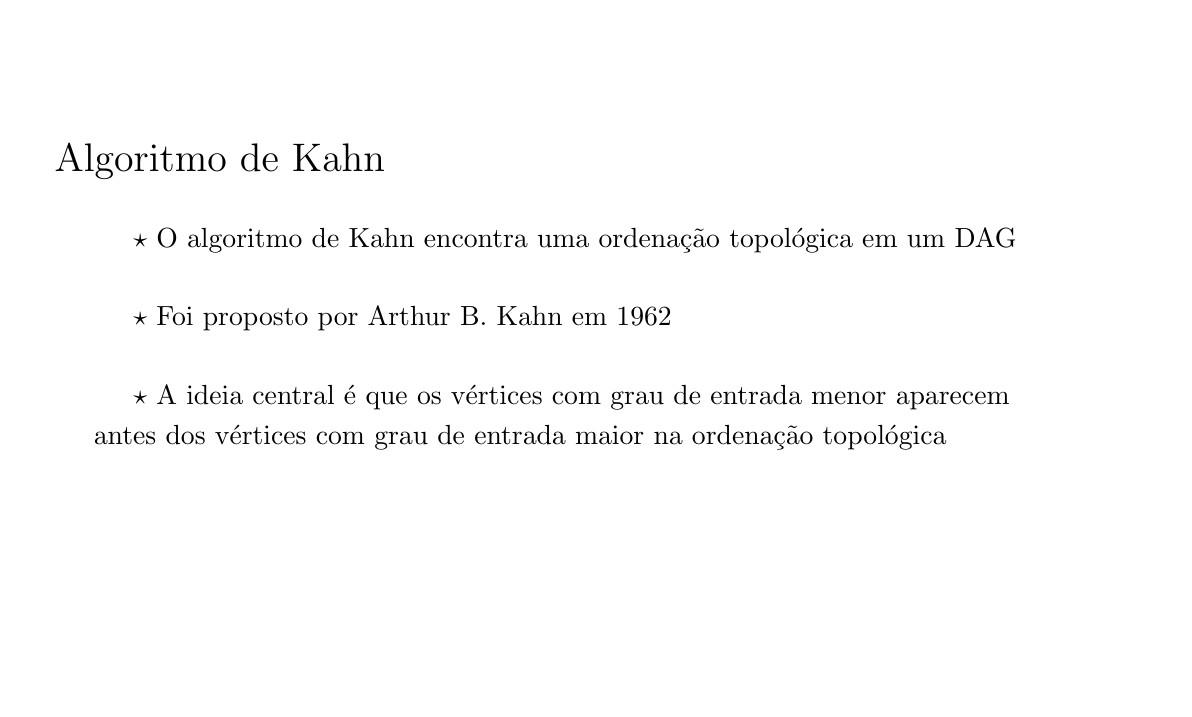
\begin{tikzpicture}
\node[draw,opacity=0] at (0, 0) {x};
\node[draw,opacity=0] at (14, 8) {x};

	\node[anchor=west] (title) at (0.0, 6.5) { \Large \bbbold{Algoritmo de Kahn} };

	\node[anchor=west] (a) at (1.0, 5.5) { $\star$ \bbtext{O algoritmo de Kahn encontra uma ordenação topológica em um DAG} };


	\node[anchor=west] (b) at (1.0, 4.5) { $\star$ \bbtext{Foi proposto por Arthur B. Kahn em 1962} };


	\node[anchor=west] (c) at (1.0, 3.5) { $\star$ \bbtext{A ideia central é que os vértices com grau de entrada menor aparecem} };

	\node[anchor=west] (c1) at (0.5, 3.0) { \bbtext{antes dos vértices com grau de entrada maior na ordenação topológica} };


\end{tikzpicture}
\end{frame}
\begin{frame}[plain,t]
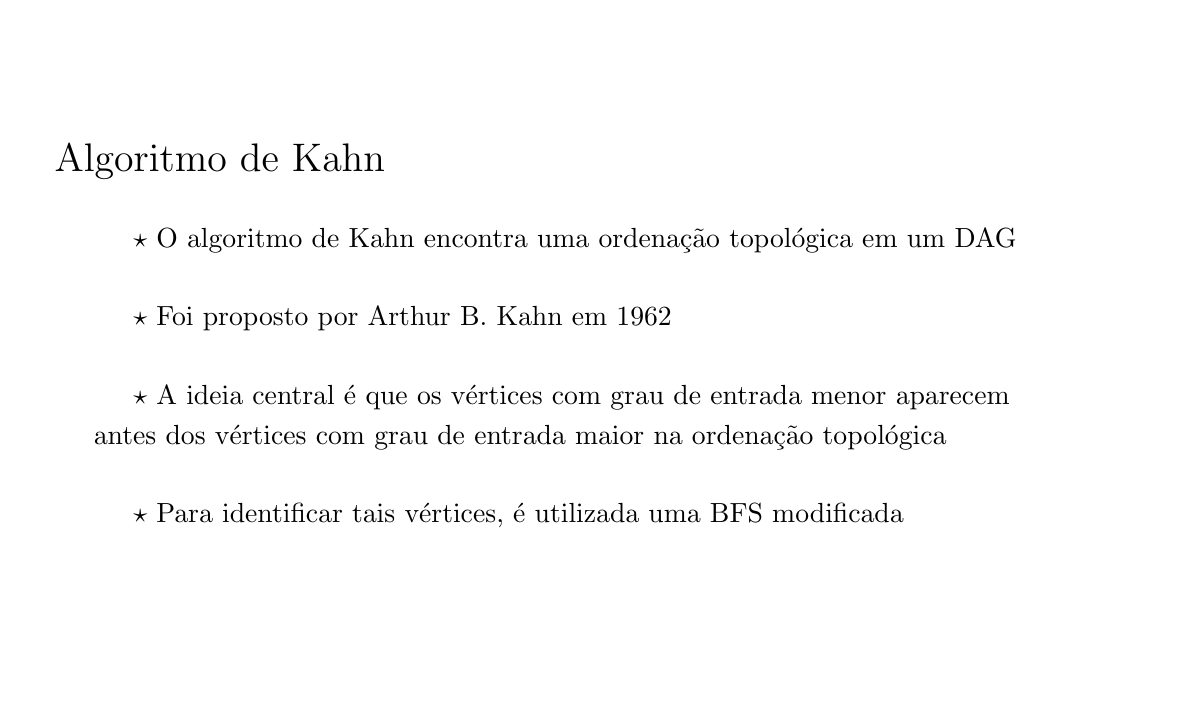
\begin{tikzpicture}
\node[draw,opacity=0] at (0, 0) {x};
\node[draw,opacity=0] at (14, 8) {x};

	\node[anchor=west] (title) at (0.0, 6.5) { \Large \bbbold{Algoritmo de Kahn} };

	\node[anchor=west] (a) at (1.0, 5.5) { $\star$ \bbtext{O algoritmo de Kahn encontra uma ordenação topológica em um DAG} };


	\node[anchor=west] (b) at (1.0, 4.5) { $\star$ \bbtext{Foi proposto por Arthur B. Kahn em 1962} };


	\node[anchor=west] (c) at (1.0, 3.5) { $\star$ \bbtext{A ideia central é que os vértices com grau de entrada menor aparecem} };

	\node[anchor=west] (c1) at (0.5, 3.0) { \bbtext{antes dos vértices com grau de entrada maior na ordenação topológica} };



	\node[anchor=west] (d) at (1.0, 2.0) { $\star$ \bbtext{Para identificar tais vértices, é utilizada uma BFS modificada} };

\end{tikzpicture}
\end{frame}
\begin{frame}[plain,t]
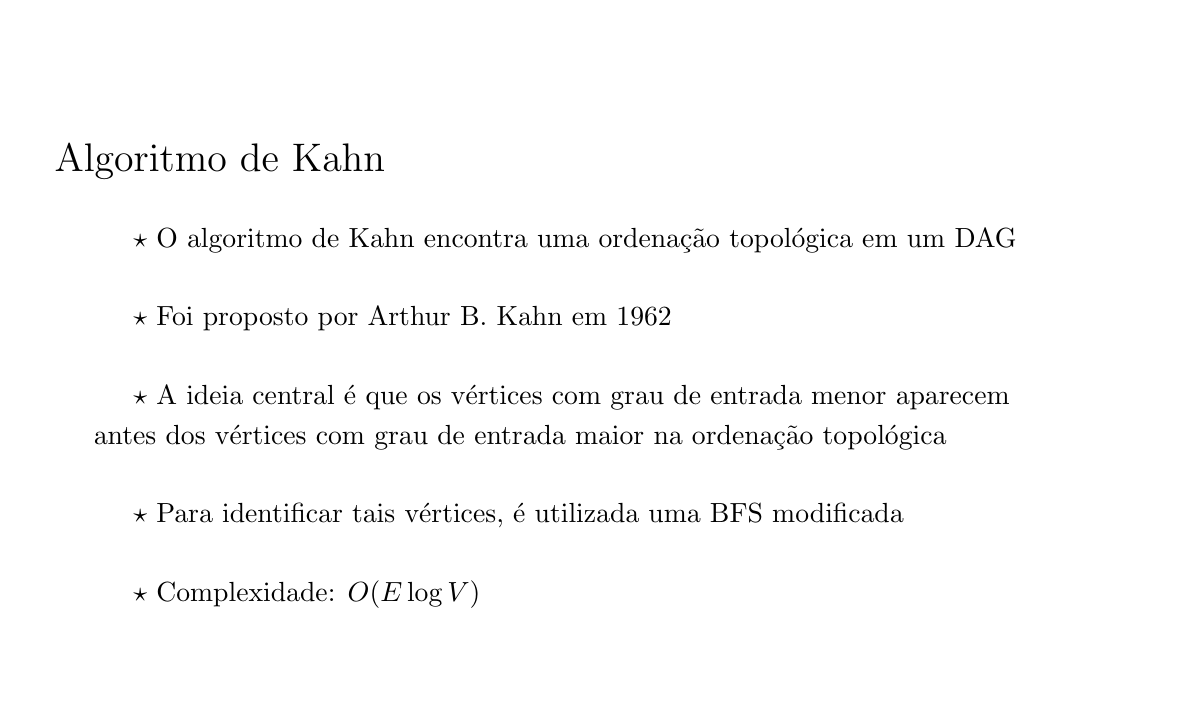
\begin{tikzpicture}
\node[draw,opacity=0] at (0, 0) {x};
\node[draw,opacity=0] at (14, 8) {x};

	\node[anchor=west] (title) at (0.0, 6.5) { \Large \bbbold{Algoritmo de Kahn} };

	\node[anchor=west] (a) at (1.0, 5.5) { $\star$ \bbtext{O algoritmo de Kahn encontra uma ordenação topológica em um DAG} };


	\node[anchor=west] (b) at (1.0, 4.5) { $\star$ \bbtext{Foi proposto por Arthur B. Kahn em 1962} };


	\node[anchor=west] (c) at (1.0, 3.5) { $\star$ \bbtext{A ideia central é que os vértices com grau de entrada menor aparecem} };

	\node[anchor=west] (c1) at (0.5, 3.0) { \bbtext{antes dos vértices com grau de entrada maior na ordenação topológica} };



	\node[anchor=west] (d) at (1.0, 2.0) { $\star$ \bbtext{Para identificar tais vértices, é utilizada uma BFS modificada} };


	\node[anchor=west] (e) at (1.0, 1.0) { $\star$ \bbtext{\bbbold{Complexidade}: $O(E\log V)$ } };

\end{tikzpicture}
\end{frame}
\begin{frame}[plain,t]
\begin{tikzpicture}
\node[draw,opacity=0] at (0, 0) {x};
\node[draw,opacity=0] at (14, 8) {x};

	\node[anchor=west] (title) at (0.0, 7.0) { \Large \bbbold{Pseudocódigo} };

\end{tikzpicture}
\end{frame}
\begin{frame}[plain,t]
\begin{tikzpicture}
\node[draw,opacity=0] at (0, 0) {x};
\node[draw,opacity=0] at (14, 8) {x};

	\node[anchor=west] (title) at (0.0, 7.0) { \Large \bbbold{Pseudocódigo} };


	\node[anchor=west] (input) at (0.5, 6.0) { \bbemph{Entrada:} \bbtext{um grafo direcionado acíclico $G(V, E)$} };

	\node[anchor=west] (output) at (0.5, 5.5) { \bbemph{Saída:} \bbtext{uma ordenação topológica $O$ de $G$} };

\end{tikzpicture}
\end{frame}
\begin{frame}[plain,t]
\begin{tikzpicture}
\node[draw,opacity=0] at (0, 0) {x};
\node[draw,opacity=0] at (14, 8) {x};

	\node[anchor=west] (title) at (0.0, 7.0) { \Large \bbbold{Pseudocódigo} };


	\node[anchor=west] (input) at (0.5, 6.0) { \bbemph{Entrada:} \bbtext{um grafo direcionado acíclico $G(V, E)$} };

	\node[anchor=west] (output) at (0.5, 5.5) { \bbemph{Saída:} \bbtext{uma ordenação topológica $O$ de $G$} };


	\node[anchor=west] (step1) at (1.0, 4.5) { $1.$ \bbtext{Insira, em uma fila $Q$, todos os vértices com grau de entrada igual a zero} };

\end{tikzpicture}
\end{frame}
\begin{frame}[plain,t]
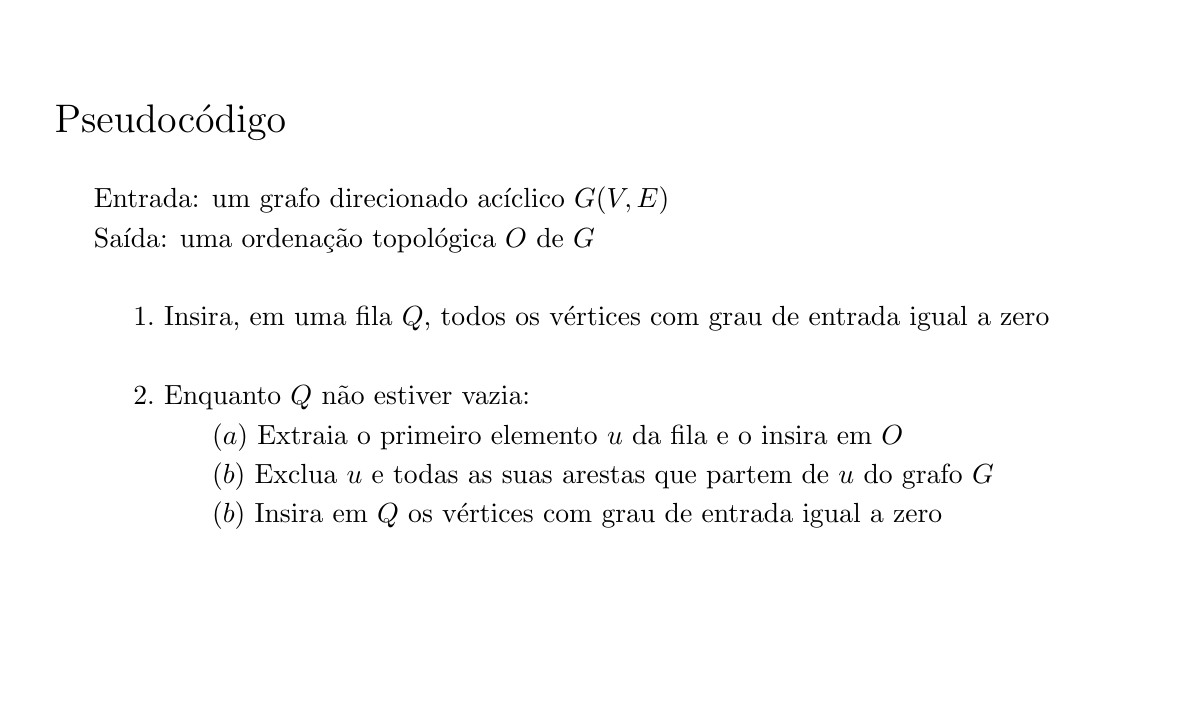
\begin{tikzpicture}
\node[draw,opacity=0] at (0, 0) {x};
\node[draw,opacity=0] at (14, 8) {x};

	\node[anchor=west] (title) at (0.0, 7.0) { \Large \bbbold{Pseudocódigo} };


	\node[anchor=west] (input) at (0.5, 6.0) { \bbemph{Entrada:} \bbtext{um grafo direcionado acíclico $G(V, E)$} };

	\node[anchor=west] (output) at (0.5, 5.5) { \bbemph{Saída:} \bbtext{uma ordenação topológica $O$ de $G$} };


	\node[anchor=west] (step1) at (1.0, 4.5) { $1.$ \bbtext{Insira, em uma fila $Q$, todos os vértices com grau de entrada igual a zero} };


	\node[anchor=west] (step2) at (1.0, 3.5) { $2.$ \bbtext{Enquanto $Q$ não estiver vazia:} };

	\node[anchor=west] (step2a) at (2.0, 3.0) { $(a)$ \bbtext{Extraia o primeiro elemento $u$ da fila e o insira em $O$} };

	\node[anchor=west] (step2b) at (2.0, 2.5) { $(b)$ \bbtext{Exclua $u$ e todas as suas arestas que partem de $u$ do grafo $G$} };

	\node[anchor=west] (step2c) at (2.0, 2.0) { $(b)$ \bbtext{Insira em $Q$ os vértices com grau de entrada igual a zero} };

\end{tikzpicture}
\end{frame}
\begin{frame}[plain,t]
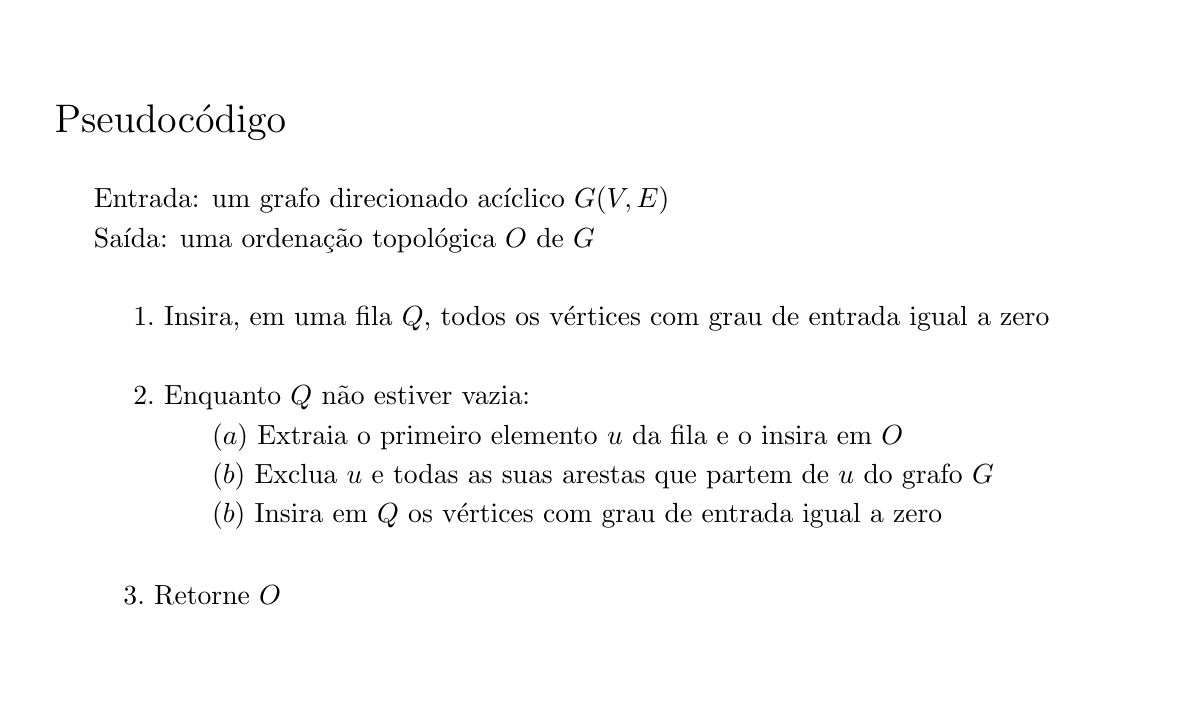
\begin{tikzpicture}
\node[draw,opacity=0] at (0, 0) {x};
\node[draw,opacity=0] at (14, 8) {x};

	\node[anchor=west] (title) at (0.0, 7.0) { \Large \bbbold{Pseudocódigo} };


	\node[anchor=west] (input) at (0.5, 6.0) { \bbemph{Entrada:} \bbtext{um grafo direcionado acíclico $G(V, E)$} };

	\node[anchor=west] (output) at (0.5, 5.5) { \bbemph{Saída:} \bbtext{uma ordenação topológica $O$ de $G$} };


	\node[anchor=west] (step1) at (1.0, 4.5) { $1.$ \bbtext{Insira, em uma fila $Q$, todos os vértices com grau de entrada igual a zero} };


	\node[anchor=west] (step2) at (1.0, 3.5) { $2.$ \bbtext{Enquanto $Q$ não estiver vazia:} };

	\node[anchor=west] (step2a) at (2.0, 3.0) { $(a)$ \bbtext{Extraia o primeiro elemento $u$ da fila e o insira em $O$} };

	\node[anchor=west] (step2b) at (2.0, 2.5) { $(b)$ \bbtext{Exclua $u$ e todas as suas arestas que partem de $u$ do grafo $G$} };

	\node[anchor=west] (step2c) at (2.0, 2.0) { $(b)$ \bbtext{Insira em $Q$ os vértices com grau de entrada igual a zero} };


	\node[] (step3) at (2.0, 1.0) { $3.$ \bbtext{Retorne $O$} };

\end{tikzpicture}
\end{frame}
\begin{frame}[plain,t]
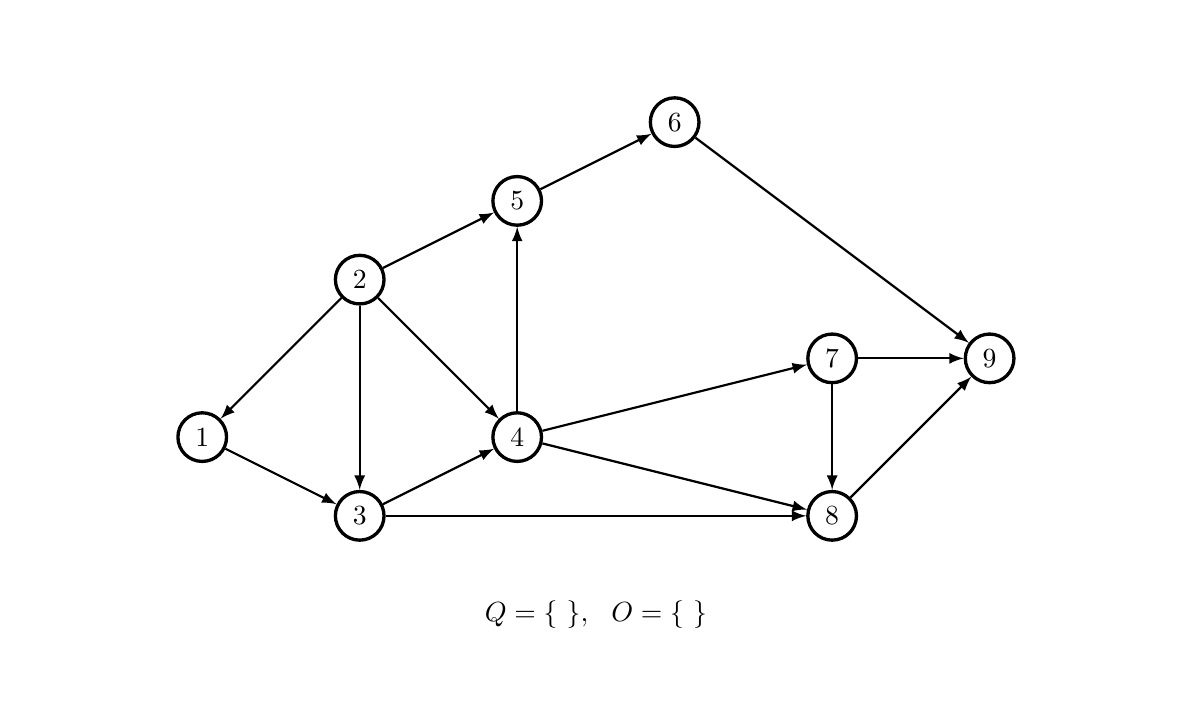
\begin{tikzpicture}
\node[draw,opacity=0] at (0, 0) {x};
\node[draw,opacity=0] at (14, 8) {x};

	\node[very thick,draw,circle] (node1) at (2.0, 3.0) { \bbtext{1} };

	\node[very thick,draw,circle] (node2) at (4.0, 5.0) { \bbtext{2} };

	\node[very thick,draw,circle] (node3) at (4.0, 2.0) { \bbtext{3} };

	\node[very thick,draw,circle] (node4) at (6.0, 3.0) { \bbtext{4} };

	\node[very thick,draw,circle] (node5) at (6.0, 6.0) { \bbtext{5} };

	\node[very thick,draw,circle] (node6) at (8.0, 7.0) { \bbtext{6} };

	\node[very thick,draw,circle] (node7) at (10.0, 4.0) { \bbtext{7} };

	\node[very thick,draw,circle] (node8) at (10.0, 2.0) { \bbtext{8} };

	\node[very thick,draw,circle] (node9) at (12.0, 4.0) { \bbtext{9} };


	\node[] (O) at (7.0, 0.75) { \bbtext{$Q = \{\ \},\ \ O = \{\ \}$} };

	\draw[thick,-latex](node2) to (node1);

	\draw[thick,-latex](node2) to (node3);

	\draw[thick,-latex](node2) to (node4);

	\draw[thick,-latex](node2) to (node5);

	\draw[thick,-latex](node1) to (node3);

	\draw[thick,-latex](node3) to (node4);

	\draw[thick,-latex](node3) to (node8);

	\draw[thick,-latex](node4) to (node5);

	\draw[thick,-latex](node4) to (node7);

	\draw[thick,-latex](node4) to (node8);

	\draw[thick,-latex](node5) to (node6);

	\draw[thick,-latex](node6) to (node9);

	\draw[thick,-latex](node7) to (node8);

	\draw[thick,-latex](node7) to (node9);

	\draw[thick,-latex](node8) to (node9);
\end{tikzpicture}
\end{frame}
\begin{frame}[plain,t]
\begin{tikzpicture}
\node[draw,opacity=0] at (0, 0) {x};
\node[draw,opacity=0] at (14, 8) {x};

	\node[very thick,draw,circle] (node1) at (2.0, 3.0) { \bbtext{1} };

	\node[very thick,draw,circle,fill=BBGreen] (node2) at (4.0, 5.0) { \bbtext{2} };

	\node[very thick,draw,circle] (node3) at (4.0, 2.0) { \bbtext{3} };

	\node[very thick,draw,circle] (node4) at (6.0, 3.0) { \bbtext{4} };

	\node[very thick,draw,circle] (node5) at (6.0, 6.0) { \bbtext{5} };

	\node[very thick,draw,circle] (node6) at (8.0, 7.0) { \bbtext{6} };

	\node[very thick,draw,circle] (node7) at (10.0, 4.0) { \bbtext{7} };

	\node[very thick,draw,circle] (node8) at (10.0, 2.0) { \bbtext{8} };

	\node[very thick,draw,circle] (node9) at (12.0, 4.0) { \bbtext{9} };


	\node[] (O) at (7.0, 0.75) { \bbtext{$Q = \{$ 2  $\},\ \ O = \{\ \}$} };

	\draw[thick,-latex](node2) to (node1);

	\draw[thick,-latex](node2) to (node3);

	\draw[thick,-latex](node2) to (node4);

	\draw[thick,-latex](node2) to (node5);

	\draw[thick,-latex](node1) to (node3);

	\draw[thick,-latex](node3) to (node4);

	\draw[thick,-latex](node3) to (node8);

	\draw[thick,-latex](node4) to (node5);

	\draw[thick,-latex](node4) to (node7);

	\draw[thick,-latex](node4) to (node8);

	\draw[thick,-latex](node5) to (node6);

	\draw[thick,-latex](node6) to (node9);

	\draw[thick,-latex](node7) to (node8);

	\draw[thick,-latex](node7) to (node9);

	\draw[thick,-latex](node8) to (node9);

\end{tikzpicture}
\end{frame}
\begin{frame}[plain,t]
\begin{tikzpicture}
\node[draw,opacity=0] at (0, 0) {x};
\node[draw,opacity=0] at (14, 8) {x};

	\node[very thick,draw,circle] (node1) at (2.0, 3.0) { \bbtext{1} };

	\node[very thick,draw,circle,fill=BBCyan] (node2) at (4.0, 5.0) { \bbtext{2} };

	\node[very thick,draw,circle] (node3) at (4.0, 2.0) { \bbtext{3} };

	\node[very thick,draw,circle] (node4) at (6.0, 3.0) { \bbtext{4} };

	\node[very thick,draw,circle] (node5) at (6.0, 6.0) { \bbtext{5} };

	\node[very thick,draw,circle] (node6) at (8.0, 7.0) { \bbtext{6} };

	\node[very thick,draw,circle] (node7) at (10.0, 4.0) { \bbtext{7} };

	\node[very thick,draw,circle] (node8) at (10.0, 2.0) { \bbtext{8} };

	\node[very thick,draw,circle] (node9) at (12.0, 4.0) { \bbtext{9} };


	\node[] (O) at (7.0, 0.75) { \bbtext{$Q = \{$  $\},\ \ O = \{$ 2 $\}$} };

	\draw[thick,-latex](node2) to (node1);

	\draw[thick,-latex](node2) to (node3);

	\draw[thick,-latex](node2) to (node4);

	\draw[thick,-latex](node2) to (node5);

	\draw[thick,-latex](node1) to (node3);

	\draw[thick,-latex](node3) to (node4);

	\draw[thick,-latex](node3) to (node8);

	\draw[thick,-latex](node4) to (node5);

	\draw[thick,-latex](node4) to (node7);

	\draw[thick,-latex](node4) to (node8);

	\draw[thick,-latex](node5) to (node6);

	\draw[thick,-latex](node6) to (node9);

	\draw[thick,-latex](node7) to (node8);

	\draw[thick,-latex](node7) to (node9);

	\draw[thick,-latex](node8) to (node9);


\end{tikzpicture}
\end{frame}
\begin{frame}[plain,t]
\begin{tikzpicture}
\node[draw,opacity=0] at (0, 0) {x};
\node[draw,opacity=0] at (14, 8) {x};

	\node[very thick,draw,circle] (node1) at (2.0, 3.0) { \bbtext{1} };


	\node[very thick,draw,circle] (node3) at (4.0, 2.0) { \bbtext{3} };

	\node[very thick,draw,circle] (node4) at (6.0, 3.0) { \bbtext{4} };

	\node[very thick,draw,circle] (node5) at (6.0, 6.0) { \bbtext{5} };

	\node[very thick,draw,circle] (node6) at (8.0, 7.0) { \bbtext{6} };

	\node[very thick,draw,circle] (node7) at (10.0, 4.0) { \bbtext{7} };

	\node[very thick,draw,circle] (node8) at (10.0, 2.0) { \bbtext{8} };

	\node[very thick,draw,circle] (node9) at (12.0, 4.0) { \bbtext{9} };


	\node[] (O) at (7.0, 0.75) { \bbtext{$Q = \{$  $\},\ \ O = \{$ 2 $\}$} };





	\draw[thick,-latex](node1) to (node3);

	\draw[thick,-latex](node3) to (node4);

	\draw[thick,-latex](node3) to (node8);

	\draw[thick,-latex](node4) to (node5);

	\draw[thick,-latex](node4) to (node7);

	\draw[thick,-latex](node4) to (node8);

	\draw[thick,-latex](node5) to (node6);

	\draw[thick,-latex](node6) to (node9);

	\draw[thick,-latex](node7) to (node8);

	\draw[thick,-latex](node7) to (node9);

	\draw[thick,-latex](node8) to (node9);



\end{tikzpicture}
\end{frame}
\begin{frame}[plain,t]
\begin{tikzpicture}
\node[draw,opacity=0] at (0, 0) {x};
\node[draw,opacity=0] at (14, 8) {x};

	\node[very thick,draw,circle,fill=BBGreen] (node1) at (2.0, 3.0) { \bbtext{1} };


	\node[very thick,draw,circle] (node3) at (4.0, 2.0) { \bbtext{3} };

	\node[very thick,draw,circle] (node4) at (6.0, 3.0) { \bbtext{4} };

	\node[very thick,draw,circle] (node5) at (6.0, 6.0) { \bbtext{5} };

	\node[very thick,draw,circle] (node6) at (8.0, 7.0) { \bbtext{6} };

	\node[very thick,draw,circle] (node7) at (10.0, 4.0) { \bbtext{7} };

	\node[very thick,draw,circle] (node8) at (10.0, 2.0) { \bbtext{8} };

	\node[very thick,draw,circle] (node9) at (12.0, 4.0) { \bbtext{9} };


	\node[] (O) at (7.0, 0.75) { \bbtext{$Q = \{$ 1 $\},\ \ O = \{$ 2 $\}$} };





	\draw[thick,-latex](node1) to (node3);

	\draw[thick,-latex](node3) to (node4);

	\draw[thick,-latex](node3) to (node8);

	\draw[thick,-latex](node4) to (node5);

	\draw[thick,-latex](node4) to (node7);

	\draw[thick,-latex](node4) to (node8);

	\draw[thick,-latex](node5) to (node6);

	\draw[thick,-latex](node6) to (node9);

	\draw[thick,-latex](node7) to (node8);

	\draw[thick,-latex](node7) to (node9);

	\draw[thick,-latex](node8) to (node9);




\end{tikzpicture}
\end{frame}
\begin{frame}[plain,t]
\begin{tikzpicture}
\node[draw,opacity=0] at (0, 0) {x};
\node[draw,opacity=0] at (14, 8) {x};

	\node[very thick,draw,circle,fill=BBCyan] (node1) at (2.0, 3.0) { \bbtext{1} };


	\node[very thick,draw,circle] (node3) at (4.0, 2.0) { \bbtext{3} };

	\node[very thick,draw,circle] (node4) at (6.0, 3.0) { \bbtext{4} };

	\node[very thick,draw,circle] (node5) at (6.0, 6.0) { \bbtext{5} };

	\node[very thick,draw,circle] (node6) at (8.0, 7.0) { \bbtext{6} };

	\node[very thick,draw,circle] (node7) at (10.0, 4.0) { \bbtext{7} };

	\node[very thick,draw,circle] (node8) at (10.0, 2.0) { \bbtext{8} };

	\node[very thick,draw,circle] (node9) at (12.0, 4.0) { \bbtext{9} };


	\node[] (O) at (7.0, 0.75) { \bbtext{$Q = \{$ $\},\ \ O = \{$ 2, 1 $\}$} };





	\draw[thick,-latex](node1) to (node3);

	\draw[thick,-latex](node3) to (node4);

	\draw[thick,-latex](node3) to (node8);

	\draw[thick,-latex](node4) to (node5);

	\draw[thick,-latex](node4) to (node7);

	\draw[thick,-latex](node4) to (node8);

	\draw[thick,-latex](node5) to (node6);

	\draw[thick,-latex](node6) to (node9);

	\draw[thick,-latex](node7) to (node8);

	\draw[thick,-latex](node7) to (node9);

	\draw[thick,-latex](node8) to (node9);





\end{tikzpicture}
\end{frame}
\begin{frame}[plain,t]
\begin{tikzpicture}
\node[draw,opacity=0] at (0, 0) {x};
\node[draw,opacity=0] at (14, 8) {x};



	\node[very thick,draw,circle] (node3) at (4.0, 2.0) { \bbtext{3} };

	\node[very thick,draw,circle] (node4) at (6.0, 3.0) { \bbtext{4} };

	\node[very thick,draw,circle] (node5) at (6.0, 6.0) { \bbtext{5} };

	\node[very thick,draw,circle] (node6) at (8.0, 7.0) { \bbtext{6} };

	\node[very thick,draw,circle] (node7) at (10.0, 4.0) { \bbtext{7} };

	\node[very thick,draw,circle] (node8) at (10.0, 2.0) { \bbtext{8} };

	\node[very thick,draw,circle] (node9) at (12.0, 4.0) { \bbtext{9} };


	\node[] (O) at (7.0, 0.75) { \bbtext{$Q = \{$ $\},\ \ O = \{$ 2, 1 $\}$} };






	\draw[thick,-latex](node3) to (node4);

	\draw[thick,-latex](node3) to (node8);

	\draw[thick,-latex](node4) to (node5);

	\draw[thick,-latex](node4) to (node7);

	\draw[thick,-latex](node4) to (node8);

	\draw[thick,-latex](node5) to (node6);

	\draw[thick,-latex](node6) to (node9);

	\draw[thick,-latex](node7) to (node8);

	\draw[thick,-latex](node7) to (node9);

	\draw[thick,-latex](node8) to (node9);






\end{tikzpicture}
\end{frame}
\begin{frame}[plain,t]
\begin{tikzpicture}
\node[draw,opacity=0] at (0, 0) {x};
\node[draw,opacity=0] at (14, 8) {x};



	\node[very thick,draw,circle,fill=BBGreen] (node3) at (4.0, 2.0) { \bbtext{3} };

	\node[very thick,draw,circle] (node4) at (6.0, 3.0) { \bbtext{4} };

	\node[very thick,draw,circle] (node5) at (6.0, 6.0) { \bbtext{5} };

	\node[very thick,draw,circle] (node6) at (8.0, 7.0) { \bbtext{6} };

	\node[very thick,draw,circle] (node7) at (10.0, 4.0) { \bbtext{7} };

	\node[very thick,draw,circle] (node8) at (10.0, 2.0) { \bbtext{8} };

	\node[very thick,draw,circle] (node9) at (12.0, 4.0) { \bbtext{9} };


	\node[] (O) at (7.0, 0.75) { \bbtext{$Q = \{$ 3 $\},\ \ O = \{$ 2, 1 $\}$} };






	\draw[thick,-latex](node3) to (node4);

	\draw[thick,-latex](node3) to (node8);

	\draw[thick,-latex](node4) to (node5);

	\draw[thick,-latex](node4) to (node7);

	\draw[thick,-latex](node4) to (node8);

	\draw[thick,-latex](node5) to (node6);

	\draw[thick,-latex](node6) to (node9);

	\draw[thick,-latex](node7) to (node8);

	\draw[thick,-latex](node7) to (node9);

	\draw[thick,-latex](node8) to (node9);







\end{tikzpicture}
\end{frame}
\begin{frame}[plain,t]
\begin{tikzpicture}
\node[draw,opacity=0] at (0, 0) {x};
\node[draw,opacity=0] at (14, 8) {x};



	\node[very thick,draw,circle,fill=BBCyan] (node3) at (4.0, 2.0) { \bbtext{3} };

	\node[very thick,draw,circle] (node4) at (6.0, 3.0) { \bbtext{4} };

	\node[very thick,draw,circle] (node5) at (6.0, 6.0) { \bbtext{5} };

	\node[very thick,draw,circle] (node6) at (8.0, 7.0) { \bbtext{6} };

	\node[very thick,draw,circle] (node7) at (10.0, 4.0) { \bbtext{7} };

	\node[very thick,draw,circle] (node8) at (10.0, 2.0) { \bbtext{8} };

	\node[very thick,draw,circle] (node9) at (12.0, 4.0) { \bbtext{9} };


	\node[] (O) at (7.0, 0.75) { \bbtext{$Q = \{$ $\},\ \ O = \{$ 2, 1, 3 $\}$} };






	\draw[thick,-latex](node3) to (node4);

	\draw[thick,-latex](node3) to (node8);

	\draw[thick,-latex](node4) to (node5);

	\draw[thick,-latex](node4) to (node7);

	\draw[thick,-latex](node4) to (node8);

	\draw[thick,-latex](node5) to (node6);

	\draw[thick,-latex](node6) to (node9);

	\draw[thick,-latex](node7) to (node8);

	\draw[thick,-latex](node7) to (node9);

	\draw[thick,-latex](node8) to (node9);








\end{tikzpicture}
\end{frame}
\begin{frame}[plain,t]
\begin{tikzpicture}
\node[draw,opacity=0] at (0, 0) {x};
\node[draw,opacity=0] at (14, 8) {x};




	\node[very thick,draw,circle] (node4) at (6.0, 3.0) { \bbtext{4} };

	\node[very thick,draw,circle] (node5) at (6.0, 6.0) { \bbtext{5} };

	\node[very thick,draw,circle] (node6) at (8.0, 7.0) { \bbtext{6} };

	\node[very thick,draw,circle] (node7) at (10.0, 4.0) { \bbtext{7} };

	\node[very thick,draw,circle] (node8) at (10.0, 2.0) { \bbtext{8} };

	\node[very thick,draw,circle] (node9) at (12.0, 4.0) { \bbtext{9} };


	\node[] (O) at (7.0, 0.75) { \bbtext{$Q = \{$ $\},\ \ O = \{$ 2, 1, 3 $\}$} };








	\draw[thick,-latex](node4) to (node5);

	\draw[thick,-latex](node4) to (node7);

	\draw[thick,-latex](node4) to (node8);

	\draw[thick,-latex](node5) to (node6);

	\draw[thick,-latex](node6) to (node9);

	\draw[thick,-latex](node7) to (node8);

	\draw[thick,-latex](node7) to (node9);

	\draw[thick,-latex](node8) to (node9);









\end{tikzpicture}
\end{frame}
\begin{frame}[plain,t]
\begin{tikzpicture}
\node[draw,opacity=0] at (0, 0) {x};
\node[draw,opacity=0] at (14, 8) {x};




	\node[very thick,draw,circle,fill=BBGreen] (node4) at (6.0, 3.0) { \bbtext{4} };

	\node[very thick,draw,circle] (node5) at (6.0, 6.0) { \bbtext{5} };

	\node[very thick,draw,circle] (node6) at (8.0, 7.0) { \bbtext{6} };

	\node[very thick,draw,circle] (node7) at (10.0, 4.0) { \bbtext{7} };

	\node[very thick,draw,circle] (node8) at (10.0, 2.0) { \bbtext{8} };

	\node[very thick,draw,circle] (node9) at (12.0, 4.0) { \bbtext{9} };


	\node[] (O) at (7.0, 0.75) { \bbtext{$Q = \{$ 4 $\},\ \ O = \{$ 2, 1, 3 $\}$} };








	\draw[thick,-latex](node4) to (node5);

	\draw[thick,-latex](node4) to (node7);

	\draw[thick,-latex](node4) to (node8);

	\draw[thick,-latex](node5) to (node6);

	\draw[thick,-latex](node6) to (node9);

	\draw[thick,-latex](node7) to (node8);

	\draw[thick,-latex](node7) to (node9);

	\draw[thick,-latex](node8) to (node9);










\end{tikzpicture}
\end{frame}
\begin{frame}[plain,t]
\begin{tikzpicture}
\node[draw,opacity=0] at (0, 0) {x};
\node[draw,opacity=0] at (14, 8) {x};




	\node[very thick,draw,circle,fill=BBCyan] (node4) at (6.0, 3.0) { \bbtext{4} };

	\node[very thick,draw,circle] (node5) at (6.0, 6.0) { \bbtext{5} };

	\node[very thick,draw,circle] (node6) at (8.0, 7.0) { \bbtext{6} };

	\node[very thick,draw,circle] (node7) at (10.0, 4.0) { \bbtext{7} };

	\node[very thick,draw,circle] (node8) at (10.0, 2.0) { \bbtext{8} };

	\node[very thick,draw,circle] (node9) at (12.0, 4.0) { \bbtext{9} };


	\node[] (O) at (7.0, 0.75) { \bbtext{$Q = \{$ $\},\ \ O = \{$ 2, 1, 3, 4 $\}$} };








	\draw[thick,-latex](node4) to (node5);

	\draw[thick,-latex](node4) to (node7);

	\draw[thick,-latex](node4) to (node8);

	\draw[thick,-latex](node5) to (node6);

	\draw[thick,-latex](node6) to (node9);

	\draw[thick,-latex](node7) to (node8);

	\draw[thick,-latex](node7) to (node9);

	\draw[thick,-latex](node8) to (node9);











\end{tikzpicture}
\end{frame}
\begin{frame}[plain,t]
\begin{tikzpicture}
\node[draw,opacity=0] at (0, 0) {x};
\node[draw,opacity=0] at (14, 8) {x};





	\node[very thick,draw,circle] (node5) at (6.0, 6.0) { \bbtext{5} };

	\node[very thick,draw,circle] (node6) at (8.0, 7.0) { \bbtext{6} };

	\node[very thick,draw,circle] (node7) at (10.0, 4.0) { \bbtext{7} };

	\node[very thick,draw,circle] (node8) at (10.0, 2.0) { \bbtext{8} };

	\node[very thick,draw,circle] (node9) at (12.0, 4.0) { \bbtext{9} };


	\node[] (O) at (7.0, 0.75) { \bbtext{$Q = \{$ $\},\ \ O = \{$ 2, 1, 3, 4 $\}$} };











	\draw[thick,-latex](node5) to (node6);

	\draw[thick,-latex](node6) to (node9);

	\draw[thick,-latex](node7) to (node8);

	\draw[thick,-latex](node7) to (node9);

	\draw[thick,-latex](node8) to (node9);











\end{tikzpicture}
\end{frame}
\begin{frame}[plain,t]
\begin{tikzpicture}
\node[draw,opacity=0] at (0, 0) {x};
\node[draw,opacity=0] at (14, 8) {x};





	\node[very thick,draw,circle,fill=BBGreen] (node5) at (6.0, 6.0) { \bbtext{5} };

	\node[very thick,draw,circle] (node6) at (8.0, 7.0) { \bbtext{6} };

	\node[very thick,draw,circle,fill=BBGreen] (node7) at (10.0, 4.0) { \bbtext{7} };

	\node[very thick,draw,circle] (node8) at (10.0, 2.0) { \bbtext{8} };

	\node[very thick,draw,circle] (node9) at (12.0, 4.0) { \bbtext{9} };


	\node[] (O) at (7.0, 0.75) { \bbtext{$Q = \{$ 5, 7 $\},\ \ O = \{$ 2, 1, 3, 4 $\}$} };











	\draw[thick,-latex](node5) to (node6);

	\draw[thick,-latex](node6) to (node9);

	\draw[thick,-latex](node7) to (node8);

	\draw[thick,-latex](node7) to (node9);

	\draw[thick,-latex](node8) to (node9);













\end{tikzpicture}
\end{frame}
\begin{frame}[plain,t]
\begin{tikzpicture}
\node[draw,opacity=0] at (0, 0) {x};
\node[draw,opacity=0] at (14, 8) {x};





	\node[very thick,draw,circle,fill=BBCyan] (node5) at (6.0, 6.0) { \bbtext{5} };

	\node[very thick,draw,circle] (node6) at (8.0, 7.0) { \bbtext{6} };

	\node[very thick,draw,circle,fill=BBGreen] (node7) at (10.0, 4.0) { \bbtext{7} };

	\node[very thick,draw,circle] (node8) at (10.0, 2.0) { \bbtext{8} };

	\node[very thick,draw,circle] (node9) at (12.0, 4.0) { \bbtext{9} };


	\node[] (O) at (7.0, 0.75) { \bbtext{$Q = \{$ 7 $\},\ \ O = \{$ 2, 1, 3, 4, 5 $\}$} };











	\draw[thick,-latex](node5) to (node6);

	\draw[thick,-latex](node6) to (node9);

	\draw[thick,-latex](node7) to (node8);

	\draw[thick,-latex](node7) to (node9);

	\draw[thick,-latex](node8) to (node9);














\end{tikzpicture}
\end{frame}
\begin{frame}[plain,t]
\begin{tikzpicture}
\node[draw,opacity=0] at (0, 0) {x};
\node[draw,opacity=0] at (14, 8) {x};






	\node[very thick,draw,circle] (node6) at (8.0, 7.0) { \bbtext{6} };

	\node[very thick,draw,circle,fill=BBGreen] (node7) at (10.0, 4.0) { \bbtext{7} };

	\node[very thick,draw,circle] (node8) at (10.0, 2.0) { \bbtext{8} };

	\node[very thick,draw,circle] (node9) at (12.0, 4.0) { \bbtext{9} };


	\node[] (O) at (7.0, 0.75) { \bbtext{$Q = \{$ 7 $\},\ \ O = \{$ 2, 1, 3, 4, 5 $\}$} };












	\draw[thick,-latex](node6) to (node9);

	\draw[thick,-latex](node7) to (node8);

	\draw[thick,-latex](node7) to (node9);

	\draw[thick,-latex](node8) to (node9);















\end{tikzpicture}
\end{frame}
\begin{frame}[plain,t]
\begin{tikzpicture}
\node[draw,opacity=0] at (0, 0) {x};
\node[draw,opacity=0] at (14, 8) {x};






	\node[very thick,draw,circle,fill=BBGreen] (node6) at (8.0, 7.0) { \bbtext{6} };

	\node[very thick,draw,circle,fill=BBGreen] (node7) at (10.0, 4.0) { \bbtext{7} };

	\node[very thick,draw,circle] (node8) at (10.0, 2.0) { \bbtext{8} };

	\node[very thick,draw,circle] (node9) at (12.0, 4.0) { \bbtext{9} };


	\node[] (O) at (7.0, 0.75) { \bbtext{$Q = \{$ 7, 6 $\},\ \ O = \{$ 2, 1, 3, 4, 5 $\}$} };












	\draw[thick,-latex](node6) to (node9);

	\draw[thick,-latex](node7) to (node8);

	\draw[thick,-latex](node7) to (node9);

	\draw[thick,-latex](node8) to (node9);
















\end{tikzpicture}
\end{frame}
\begin{frame}[plain,t]
\begin{tikzpicture}
\node[draw,opacity=0] at (0, 0) {x};
\node[draw,opacity=0] at (14, 8) {x};






	\node[very thick,draw,circle,fill=BBGreen] (node6) at (8.0, 7.0) { \bbtext{6} };

	\node[very thick,draw,circle,fill=BBCyan] (node7) at (10.0, 4.0) { \bbtext{7} };

	\node[very thick,draw,circle] (node8) at (10.0, 2.0) { \bbtext{8} };

	\node[very thick,draw,circle] (node9) at (12.0, 4.0) { \bbtext{9} };


	\node[] (O) at (7.0, 0.75) { \bbtext{$Q = \{$ 6 $\},\ \ O = \{$ 2, 1, 3, 4, 5, 7 $\}$} };












	\draw[thick,-latex](node6) to (node9);

	\draw[thick,-latex](node7) to (node8);

	\draw[thick,-latex](node7) to (node9);

	\draw[thick,-latex](node8) to (node9);

















\end{tikzpicture}
\end{frame}
\begin{frame}[plain,t]
\begin{tikzpicture}
\node[draw,opacity=0] at (0, 0) {x};
\node[draw,opacity=0] at (14, 8) {x};






	\node[very thick,draw,circle,fill=BBGreen] (node6) at (8.0, 7.0) { \bbtext{6} };


	\node[very thick,draw,circle] (node8) at (10.0, 2.0) { \bbtext{8} };

	\node[very thick,draw,circle] (node9) at (12.0, 4.0) { \bbtext{9} };


	\node[] (O) at (7.0, 0.75) { \bbtext{$Q = \{$ 6 $\},\ \ O = \{$ 2, 1, 3, 4, 5, 7 $\}$} };












	\draw[thick,-latex](node6) to (node9);



	\draw[thick,-latex](node8) to (node9);


















\end{tikzpicture}
\end{frame}
\begin{frame}[plain,t]
\begin{tikzpicture}
\node[draw,opacity=0] at (0, 0) {x};
\node[draw,opacity=0] at (14, 8) {x};






	\node[very thick,draw,circle,fill=BBGreen] (node6) at (8.0, 7.0) { \bbtext{6} };


	\node[very thick,draw,circle,fill=BBGreen] (node8) at (10.0, 2.0) { \bbtext{8} };

	\node[very thick,draw,circle] (node9) at (12.0, 4.0) { \bbtext{9} };


	\node[] (O) at (7.0, 0.75) { \bbtext{$Q = \{$ 6, 8 $\},\ \ O = \{$ 2, 1, 3, 4, 5, 7 $\}$} };












	\draw[thick,-latex](node6) to (node9);



	\draw[thick,-latex](node8) to (node9);



















\end{tikzpicture}
\end{frame}
\begin{frame}[plain,t]
\begin{tikzpicture}
\node[draw,opacity=0] at (0, 0) {x};
\node[draw,opacity=0] at (14, 8) {x};






	\node[very thick,draw,circle,fill=BBCyan] (node6) at (8.0, 7.0) { \bbtext{6} };


	\node[very thick,draw,circle,fill=BBGreen] (node8) at (10.0, 2.0) { \bbtext{8} };

	\node[very thick,draw,circle] (node9) at (12.0, 4.0) { \bbtext{9} };


	\node[] (O) at (7.0, 0.75) { \bbtext{$Q = \{$ 8 $\},\ \ O = \{$ 2, 1, 3, 4, 5, 7, 6 $\}$} };












	\draw[thick,-latex](node6) to (node9);



	\draw[thick,-latex](node8) to (node9);




















\end{tikzpicture}
\end{frame}
\begin{frame}[plain,t]
\begin{tikzpicture}
\node[draw,opacity=0] at (0, 0) {x};
\node[draw,opacity=0] at (14, 8) {x};








	\node[very thick,draw,circle,fill=BBGreen] (node8) at (10.0, 2.0) { \bbtext{8} };

	\node[very thick,draw,circle] (node9) at (12.0, 4.0) { \bbtext{9} };


	\node[] (O) at (7.0, 0.75) { \bbtext{$Q = \{$ 8 $\},\ \ O = \{$ 2, 1, 3, 4, 5, 7, 6 $\}$} };















	\draw[thick,-latex](node8) to (node9);





















\end{tikzpicture}
\end{frame}
\begin{frame}[plain,t]
\begin{tikzpicture}
\node[draw,opacity=0] at (0, 0) {x};
\node[draw,opacity=0] at (14, 8) {x};








	\node[very thick,draw,circle,fill=BBCyan] (node8) at (10.0, 2.0) { \bbtext{8} };

	\node[very thick,draw,circle] (node9) at (12.0, 4.0) { \bbtext{9} };


	\node[] (O) at (7.0, 0.75) { \bbtext{$Q = \{$ $\},\ \ O = \{$ 2, 1, 3, 4, 5, 7, 6, 8 $\}$} };















	\draw[thick,-latex](node8) to (node9);






















\end{tikzpicture}
\end{frame}
\begin{frame}[plain,t]
\begin{tikzpicture}
\node[draw,opacity=0] at (0, 0) {x};
\node[draw,opacity=0] at (14, 8) {x};









	\node[very thick,draw,circle] (node9) at (12.0, 4.0) { \bbtext{9} };


	\node[] (O) at (7.0, 0.75) { \bbtext{$Q = \{$ $\},\ \ O = \{$ 2, 1, 3, 4, 5, 7, 6, 8 $\}$} };






































\end{tikzpicture}
\end{frame}
\begin{frame}[plain,t]
\begin{tikzpicture}
\node[draw,opacity=0] at (0, 0) {x};
\node[draw,opacity=0] at (14, 8) {x};









	\node[very thick,draw,circle,fill=BBGreen] (node9) at (12.0, 4.0) { \bbtext{9} };


	\node[] (O) at (7.0, 0.75) { \bbtext{$Q = \{$ 9 $\},\ \ O = \{$ 2, 1, 3, 4, 5, 7, 6, 8 $\}$} };







































\end{tikzpicture}
\end{frame}
\begin{frame}[plain,t]
\begin{tikzpicture}
\node[draw,opacity=0] at (0, 0) {x};
\node[draw,opacity=0] at (14, 8) {x};









	\node[very thick,draw,circle,fill=BBCyan] (node9) at (12.0, 4.0) { \bbtext{9} };


	\node[] (O) at (7.0, 0.75) { \bbtext{$Q = \{$ $\},\ \ O = \{$ 2, 1, 3, 4, 5, 7, 6, 8, 9 $\}$} };








































\end{tikzpicture}
\end{frame}
\begin{frame}[plain,t]
\begin{tikzpicture}
\node[draw,opacity=0] at (0, 0) {x};
\node[draw,opacity=0] at (14, 8) {x};











	\node[] (O) at (7.0, 0.75) { \bbtext{$Q = \{$ $\},\ \ O = \{$ 2, 1, 3, 4, 5, 7, 6, 8, 9 $\}$} };









































\end{tikzpicture}
\end{frame}
\begin{frame}[plain,t]

\inputsnippet{cpp}{10}{24}{codes/kahn.cpp}

\end{frame}
\begin{frame}[plain,t]

\inputsnippet{cpp}{26}{36}{codes/kahn.cpp}

\end{frame}
\begin{frame}[plain,t]
\begin{tikzpicture}
\node[draw,opacity=0] at (0, 0) {x};
\node[draw,opacity=0] at (14, 8) {x};

	\node[anchor=west] (title) at (0.0, 6.0) { \Large \bbbold{Problemas sugeridos} };

	\node[anchor=west] (a) at (1.0, 5.0) { $1.$ \bbtext{Codeforces 510C -- Fox and Names} };

	\node[anchor=west] (b) at (1.0, 4.0) { $2.$ \bbtext{OJ 11060 -- Beverages} };

	\node[anchor=west] (c) at (1.0, 3.0) { $3.$ \bbtext{SPOJ TOPOSORT -- Topological Sorting} };

	\node[anchor=west] (d) at (1.0, 2.0) { $4.$ \bbtext{Timus 1280 -- Topological Sorting} };

\end{tikzpicture}
\end{frame}
\begin{frame}[plain,t]
\begin{tikzpicture}
\node[draw,opacity=0] at (0, 0) {x};
\node[draw,opacity=0] at (14, 8) {x};

	\node[anchor=west] (title) at (0.0, 6.5) { \Large \bbbold{Referências} };

	\node[anchor=west] (a) at (1.0, 5.5) { $1.$ \bbtext{\bbbold{ACM Digital Library}. \bbenglish{Topological sorting of large networks}, A. B. Kahn, 1962.} };

	\node[anchor=west] (b) at (1.0, 4.5) { $2.$ \bbbold{HALIM}, \bbtext{Felix}; \bbbold{HALIM}, \bbtext{Steve}. \bbenglish{Competitive Programming 3,} \bbtext{2010.} };

	\node[anchor=west] (c) at (1.0, 3.5) { $3.$ \bbbold{LAAKSONEN}, \bbtext{Antti}. \bbenglish{Competitive Programmer's Handbook,} \bbtext{2018.} };

	\node[anchor=west] (d) at (1.0, 2.5) { $4.$ \bbbold{Wikipédia}. \bbenglish{Robert Tarjan,} \bbtext{acesso em 08/09/2021.} };

	\node[anchor=west] (e) at (1.0, 1.5) { $5.$ \bbbold{Wikipédia}. \bbenglish{Topological sorting,} \bbtext{acesso em 08/09/2021.} };

\end{tikzpicture}
\end{frame}
\end{document}
